\documentclass[12pt]{report}
\usepackage{multirow}
\usepackage{rotating}
\usepackage{hhline}
\usepackage[]{graphicx}
\usepackage[left=1.25in, right=1in,top=1in,bottom=1in,headheight=6pt, a4paper]{geometry}
\usepackage{titling}
\usepackage{booktabs}
\usepackage{natbib}
\usepackage{url}
% \usepackage{biblatex}
% \usepackage{times}

\usepackage{microtype}
\usepackage[utf8x]{inputenc}
\usepackage{xcolor}
\usepackage{datetime2}

\usepackage{enumitem}
\usepackage[font=normalsize,tableposition=top]{caption}
\usepackage{etoolbox}\usepackage{setspace}
\usepackage[explicit]{}
\usepackage{algpseudocode, algorithm}
\usepackage{amsmath}
\usepackage{amsfonts}
\usepackage{amssymb}
\usepackage{hyperref}
\usepackage{pgfgantt}
\usepackage{adjustbox}
\usepackage{multicol}
\usepackage{mathptmx}
\usepackage{titlesec}
\usepackage{setspace}
\usepackage{import}
\usepackage{enumitem}
\usepackage{bm}
\usepackage{amsmath, amsfonts}
\usepackage{pdflscape}
\usepackage{everypage-1x}
\usepackage{wrapfig}
\usepackage{scrextend}
\usepackage{etoolbox}
\usepackage{appendix}
\usepackage{ragged2e}
\usepackage{tabularx}


\usepackage{listings}


\definecolor{dkgreen}{rgb}{0,0.6,0}
\definecolor{gray}{rgb}{0.5,0.5,0.5}
\definecolor{mauve}{rgb}{0.58,0,0.82}



\newcolumntype{Y}{>{\raggedright\arraybackslash}X}



\renewcommand\appendixtocname{APPENDIX}
\renewcommand\appendixpagename{APPENDIX}
\renewcommand{\bibname}{REFERENCES}

%\usetikzlibrary{positioning}
% \ganttset{group/.append style={orange},
% milestone/.append style={red},
% progress label node anchor/.append style={text=red}}

\linespread{1.3}
\setlength{\parskip}{6pt}
\setlength{\parindent}{0em}


%--------------------



%------ SET DOCUMENT GEOMETRY ------%
\usepackage{geometry}
\geometry{a4paper, left=1.25in, top=1in, bottom=1in, right=1in}


%------ FORMAT CHAPTER, SECTION, AND SUBSECTION TITLE ------%
  \titleformat{\chapter}{
  \normalfont\fontsize{16}{15}\bfseries
  }{\thechapter}{1em}{}

  \titleformat{\section}{
  \normalfont\fontsize{14}{15}\bfseries
  }{\thesection}{1em}{}

  \titleformat{\subsection}{
  \normalfont\fontsize{12}{15}\bfseries
  }{\thesubsection}{1em}{}

  \titlespacing{\chapter}{0pt}{-0.5in}{-0.5em}
  \titlespacing{\section}{0pt}{0pt}{-1em}
  \titlespacing{\subsection}{0pt}{0pt}{-1em}


%------ SET SPACING AND INDENTS ------%
\renewcommand{\baselinestretch}{1.5} 
\setlength{\parindent}{0pt}
\setlength{\parskip}{12pt}


%------ SETUP LINKS ------%
\usepackage{hyperref}
\hypersetup{
    colorlinks,
    citecolor=black,
    filecolor=black,
    linkcolor=black,
    urlcolor=black
}


%------ FORMAT TABLE OF CONTENTS ------%
\usepackage{tocloft}


\cftsetindents{section}{1.4em}{1.75em}
\cftsetindents{subsection}{3.2em}{2.6em}
\setlength{\cftbeforetoctitleskip}{-2.5em}
\setlength{\cftbeforechapskip}{0.25em}

\renewcommand{\cftchapleader}{\dotfill}

\renewcommand{\cftdotsep}{1.5}
\renewcommand{\cftsecfont}{\normalfont}
\renewcommand{\cftsecpagefont}{\normalfont}

\setlength{\cftbeforeloftitleskip}{-2.5em}
\setlength{\cftbeforelottitleskip}{-2.5em}

\setlength{\cftfigindent}{0pt}
\setlength{\cfttabindent}{0pt}

\renewcommand{\cftfigfont}{Figure }
\renewcommand{\cfttabfont}{Table }


%------ FORMAT TABLE CAPTIONS ------%
\usepackage{caption} 
\captionsetup[table]{skip=10pt}
\captionsetup[figure]{labelfont=bf,textfont=bf}
\captionsetup[table]{labelfont=bf,textfont=bf}


\newcommand{\Lpagenumber}{\ifdim\textwidth=\linewidth\else\bgroup
  \dimendef\margin=0 %use \margin instead of \dimen0
  \ifodd\value{page}\margin=\oddsidemargin
  \else\margin=\evensidemargin
  \fi
  \raisebox{\dimexpr -\topmargin-\headheight-\headsep-0.5\linewidth}[0pt][0pt]{%
    \rlap{\hspace{\dimexpr \margin+\textheight+\footskip}%
    \llap{\rotatebox{90}{\thepage}}}}%
\egroup\fi}
\AddEverypageHook{\Lpagenumber}%


\newcommand{\theinstitute}{Faculty of Humanities and Social Sciences }
\newcommand{\thecampus}{Lalitpur Engineering College }
\newcommand{\thedepartment}{Department of Computer Application }
\newcommand{\thedepartmentAddress}{Lalitpur, Nepal }
\newcommand{\thedepartmentFullAddress}{Patan, Lalitpur, Nepal }
\newcommand{\theprogramcoordinator}{Er. Bibat Thokar }
\newcommand{\theHOD}{Er.Bibat Thokar }
\newcommand{\authorWithAnd}{ Sushant Bramhacharya (LEC077BCA08) and Amit Maharjan (LEC077BCA01)}


\title{Code Connect : Connect with Creatives}
\author{ Sushant Bramhacharya (LEC077BCA08)\\Amit Maharjan (LEC077BCA01) }
\newcommand{\theroll}{
  % LEC077BCA01\\LEC077BCA08
}
\date{October, 2023}
\newcommand{\thesupervisor}{Er. Sandesh Sharan Poudel}


\linespread{1.5}
\begin{document}

\pagenumbering{roman}

\thispagestyle{empty}
\begin{center}
\begin{spacing}{1.6}


\includegraphics[scale=0.20]{img/Graphics/lec.jpg}

\textbf{
\large{TRIBHUVAN UNIVERSITY}\\
\MakeUppercase{\large{\theinstitute}}\\
\MakeUppercase{\large{\thecampus}}}

\vspace{0.5cm}

\hspace{-8cm}
% \textbf{PROJECT NO.: \theroll}

\vspace{0.5cm}

\textbf{\MakeUppercase{\thetitle}\\
\vspace{0.5cm} 
BY \\ 
\MakeUppercase{\theauthor}}

\vspace{0.5cm}

\textbf{FINAL REPORT\\
SUBMITTED TO THE \MakeUppercase{\thedepartment}\\ IN PARTIAL FULFILLMENT OF THE REQUIREMENT FOR\\ THE DEGREE OF BACHELORS IN COMPUTER APPLICATION}
\bigskip

\par
\textbf{\MakeUppercase{\thedepartment}}\\
\textbf{\MakeUppercase{\thedepartmentAddress}}
\vspace{1cm}

\textbf{\MakeUppercase{\thedate}}


\end{spacing}
\end{center}

\clearpage
\begin{center}
\begin{spacing}{1.6}
\thispagestyle{empty}


\includegraphics[scale=0.25]{img/Graphics/TUlogo.png}

\textbf{
\large{Tribhuvan University}\\
\large{\theinstitute}}\\
\vspace{0.5cm}
\textbf{\MakeUppercase{\thetitle}\\
\vspace{0.5cm} 
Submitted to\\ 
\thedepartment\\
\thecampus}\\
\vspace{0.5cm}

\textbf{In partial fulfillment of the requirement for the degree of Bachelors in Computer Application}
\bigskip

\par

\textbf{
Submitted by\\
\theauthor\\
\MakeUppercase{\thedate}}\\
\vspace{1cm}
\textbf{
Under the Coordination of\\
\thesupervisor
}
\end{spacing}
\end{center}

\clearpage
% \chapter*{\centerline{DECLARATION}}
\addcontentsline{toc}{chapter}{DECLARATION}
\vspace{-0.5cm}
I declare that the work hereby submitted for Bachelors in Computer Application at the \thedepartment, \thecampus \ entitled "\textbf{\thetitle}" is my own work and has not been previously submitted by
me at any university for any academic award.
I authorize the \thedepartment, \thecampus \ to lend this project work
to other institutions or individuals for the purpose of scholarly research.

\vspace{1cm}

\textbf{\theauthor} \\
\theroll \\
\thedate
\newgeometry{left=1.5in, top=2.5in, bottom=1in, right=1in}
\chapter*{\centerline{RECOMMENDATION}}
\addcontentsline{toc}{chapter}{RECOMMENDATION}
\vspace{-0.5cm}
The undersigned certify that they have read and recommend to the \thedepartment \ for acceptance, a project work entitled “\textbf{\thetitle}”, submitted by \textbf{\authorWithAnd} in partial fulfillment of the requirement
for the award of the degree of “\textbf{Bachelors in Computer Application}”.

\vspace{1cm}
\rule{0.5\textwidth}{0.4pt}\\
\textbf{Project Coordinator}\\
\thesupervisor\\
Lecturer\\
\thedepartment, Lalitpur Engineering College\\

\vspace{1cm}
\rule{0.5\textwidth}{0.4pt}\\
\textbf{BCA Program Coordinator}\\
\theprogramcoordinator\\
Lecturer\\
\thedepartment, \thecampus\\

\vspace{1cm}
\thedate
\restoregeometry 
\newgeometry{left=1.5in, top=2.5in, bottom=1in, right=1in}
\chapter*{\centerline{DEPARTMENTAL ACCEPTANCE}}
\addcontentsline{toc}{chapter}{DEPARTMENTAL ACCEPTANCE}
\vspace{-0.5cm}
The project work entitled “\textbf{\thetitle}”, submitted by \textbf {\authorWithAnd }in
partial fulfillment of the requirement for the award of the degree of “\textbf{Bachelors of Computer Application}” has been accepted as
a genuine record of work independently carried out by the students in the department.

\vspace{5cm}

\begin{addmargin}[5.5cm]{0em}
\rule{0.62\textwidth}{0.4pt}\\
\textbf{\theHOD}\\
BCA Program Coordinator\\
\thedepartment,\\
\thecampus,\\
\theinstitute,\\
Tribhuvan University,
Nepal.\\
\end{addmargin}

\vspace{2cm}

\thedate

\restoregeometry % Approval letter
\begin{figure}
    \centering
    
\includegraphics[width=1.25in]{img/Graphics/TUlogo.png}
\end{figure}
\begin{center}
    {\fontsize{14pt}{18}\selectfont
    \textbf{Tribhuvan University\\
    Faculty of Humanities and Social Sciences\\
    Lalitpur Engineering College\\
    \vspace{0.2in}
    LETTER OF APPROVAL\\}
    \vspace{0.2in}}
\end{center}
This is to certify that this project prepared by Amit Maharjan and Sushant Bramhacharya entitled “\textbf{Code Connect :  Connect with Creatives}” in partial fulfillment of the requirements for the degree of Bachelor in Computer Application has been evaluated. In our opinion it is satisfactory in the
scope and quality as a project for the required degree.\\
\begin{center}
    {\fontsize{14pt}{18}\selectfont
    \vspace{0.1in}
    \begin{table}[ht]
        \begin{tabularx}{\textwidth}{|Y|Y|}
        \hline
        &\\
        &\\
        \textbf{SIGNATURE of Supervisor}&\textbf{SIGNATURE of Coordinator}\\
        &\\
        &\\
        Er Sandesh Saran Poudel & Er Bibat Thokar \\
        Project Supervisor & BCA Program Coordinator \\
        Department of Computer Application & Department of Computer Application\\
        Lalitpur Engineering College & Lalitpur Engineering College \\
        &\\
        &\\
        \hline
        &\\
        \textbf{SIGNATURE of Internal Examiner}&\textbf{SIGNATURE of External Examiner}\\
        &\\
        &\\
        \hline
        \end{tabularx}
        \end{table}
        
    
    }
\end{center}
\chapter*{\centerline{ACKNOWLEDGMENT}}
\addcontentsline{toc}{chapter}{ACKNOWLEDGMENT}
\vspace{-0.5cm}
This project work would not have been possible without the guidance and the help of
several individuals who in one way or another contributed and extended their
valuable assistance in the preparation and completion of this study.


First of all, I would like to express my sincere gratitude to my supervisor, \textbf{\thesupervisor}, of \textbf{(Organization))} for providing invaluable guidance, insightful comments, meticulous suggestions, and encouragement throughout the duration of
this project work. My sincere thanks also goes to the BCA coordinator, \textbf{\theprogramcoordinator}, for coordinating the project works, providing astute criticism, and having
inexhaustible patience.

\textbf{[Include a few lines of appreciation if assistance was received from organizations
or individuals other than the supervisor]}

I am also grateful to my classmates and friends for offering me advice and moral
support. To my family, thank you for encouraging me in all of my pursuits and
inspiring me to follow my dreams. I am especially grateful to my parents, who
supported me emotionally, believed in me and wanted the best for me.

\vspace{1cm}

\textbf{\theauthor} \\
\theroll \\
\thedate
%==============================Abstract Page=================================================
\chapter*{\centerline{ABSTRACT}}
\addcontentsline{toc}{chapter}{ABSTRACT}
\thispagestyle{plain} 
% Abstract (200 to 250 Words)
\vspace{-0.5cm}

Code Connect is a revolutionary social media platform made specifically to the needs of programmers and developers. With a focus on collaboration, knowledge sharing, and networking, Code Connect serves as an interactive space where programmers can connect with like-minded individuals, exchange ideas, and explore new opportunities within the coding community.
The platform offers a user-friendly interface and a range of features designed to enhance the programmer's experience. Users can create personalized profiles to showcase their skills, experiences, and projects, attracting potential collaborators or employers. A comprehensive search and recommendation system allows users to discover discussions tailored to their interests and preferences.

One of Code Connect's unique strengths is Messaging system. Real-time messaging facilitates productive discussions and timely feedback among peers.
Furthermore, Code Connect encourages the sharing of code snippets, problems, and open-source projects. Users can publish their code, receive feedback, and collaborate on improvements, building a valuable repository of shared resources accessible to the entire coding community.

In conclusion, Code Connect is a vital platform that connects programmers, fosters collaboration, and facilitates growth within the coding community. By empowering programmers to share knowledge, explore opportunities, and connect with peers, Code Connect aims to advance the programming industry as a whole both for newcomers and advanced ones.
\\\\
\textbf{Keywords:}  Connection, Customized Profile, Discussion and  Messaging
%=============================================================================================
% (a) Inclusion of three to four Keywords (Lexicographical Order)
\newpage



%=================TOC=========================================================================

\cftsetindents{section}{1.5em}{2.1em}
\cftsetindents{subsection}{3.6em}{3.1em}

\chapter*{\centerline{TABLE OF CONTENTS}}
\addcontentsline{toc}{chapter}{TABLE OF CONTENTS}
\def\contentsname{\empty}
\tableofcontents
\clearpage




\chapter*{\centerline{LIST OF FIGURES}}
\addcontentsline{toc}{chapter}{LIST OF FIGURES}
\def\listfigurename{\empty}
\newcommand*{\noaddvspace}{\renewcommand*{\addvspace}[1]{}}
\addtocontents{lof}{\protect\noaddvspace}
\listoffigures
\clearpage



\chapter*{\centerline{LIST OF TABLES}}
\addcontentsline{toc}{chapter}{LIST OF TABLES}
\def\listtablename{\empty}
\addtocontents{lot}{\protect\noaddvspace}
\listoftables
\clearpage




%================Abbreviation Page=====================================
\chapter*{\centerline{LIST OF ABBREVIATIONS}}
\addcontentsline{toc}{chapter}{LIST OF ABBREVIATIONS}

% ABBR\hspace:   ABBREVIATIONS\\



\begin{tabular}{l@{\hspace{3cm}}p{15cm}}
  ACID & Atomicity, Consistency, Isolation, Durability \\
  BSD & Berkeley Software Distribution \\
  CMS & Content Management System \\
  CV & Curriculum Vitae \\
  CSS & Cascading Style Sheets \\
  DFD & Data Flow Diagram \\
  DOM & Document Object Model \\
  ER & Entity-Relationship \\
  HTML & Hypertext Markup Language \\
  IT & Information Technology \\
  JS & JavaScript \\
  MySQL & My Structured Query Language \\
  OS & Operating System \\
  PHP & Hypertext Preprocessor \\
  SQL & Structured Query Language \\
  UI & User Interface \\
  UML & Unified Modeling Language \\
  URL & Uniform Resource Locator \\
  UX & User Experience \\

\end{tabular}

%===============================================================================



% \newpage
%=============================================================================


\pagenumbering{arabic}

%=====================Report Body=============================================


\chapter{INTRODUCTION}
% (20% of Proposal Length)
\pagenumbering{arabic}

% Introduction: (20\% of Report Length)


\section{Introduction}

Code Connect serves as a social media hub tailored to the needs of IT enthusiast, aiming to fill the void of specialized functionalities on current social platforms. This unique platform provides a designated arena where IT professionals can unite, cooperate, and gain access to their own soical network.
\section{Problem Statement}

There are many general social media platforms available, but none of them are specifically designed for IT professionals. This means that IT professionals often have to use general platforms, which can be less effective for networking and collaboration.
Most general social media platforms do not have dedicated spaces for IT professionals to share their resumes. This can make it difficult for IT professionals to get their resumes seen by potential employers.
There are no specific resume management tools available for IT professionals. This means that IT professionals often have to use general resume management tools, which can be less effective for managing IT-related resumes.

There is no specific portfolio management tool available for IT professionals. This means that IT professionals often have to use general portfolio management tools, which can be less effective for managing IT-related portfolios.
IT professionals are often underrepresented in other social media platforms. This can make it difficult for IT professionals to reach a wider audience and connect with other IT professionals.
The challenges listed above can be even more difficult for new aspiring IT professionals. This is because new IT professionals may not have the same level of experience or connections as more experienced IT professionals.
\section{Objectives}
\begin{itemize}
  \item To create a social media having normal functionalities and extra specifically  for creative it professionals.
\end{itemize}
\section{Scope and Limitations}
The app should provide a space for IT professionals to network with each other. This could be done through discussions or Messaging. Networking can help IT professionals to discover jobs, learn new skills, and stay up-to-date on the latest trends.
The app should make it easy for new comers in field of IT.
The app should offer a nice way to showcase their skill and projects.
The app should have code snippets sharing and discussion.
The app should have connection functions for connecting between peers, friends and seniors.
\section{Limitation}
\begin{itemize}
    \item Our system doesnt have more interactive message system.
    \item Videos Cannot be Uploaded.
    \item Our system does not have a robust notification system. Users are only notified when they receive a new message or when someone geeks or comments on their post.
\end{itemize}

\section{Potential applications}
\begin{itemize}
    \item \textbf{Networking and Collaboration}: IT professionals can connect with peers, mentors, and industry experts, fostering collaborations on projects, sharing insights, and expanding their professional network.
    \item \textbf{Skill Development}: Code Connect can share codes regarding to their problems and projects.
    \item \textbf{Knowledge Sharing}: Members can share code and resources related to programming languages, frameworks, tools, and best practices.
    \item \textbf{Problem Solving}: People can comment on problems stating solutions.  
    \item \textbf{Messaging}: They can use code connect messenger to have private conversations.
  \end{itemize}
\section{Originality of Project}

\begin{itemize}
    \item \textbf{Specialized Platform}: Code Connect stands out by being a social media platform specifically designed for IT professionals, acknowledging their distinct requirements and expertise.
    \item \textbf{Unique Needs}: The project pioneers by recognizing and addressing the unique challenges and aspirations that IT professionals encounter in their career paths, setting it apart from more generalized social networks.
    \item \textbf{Career Enhancement}: Code Connect provides tools like specialized resume and portfolio management, facilitating the effective representation of IT professionals' skills and experiences to potential employers and collaborators.
    \item \textbf{Empowerment and Growth}: Through Code Connect, IT professionals are empowered to connect, learn, collaborate, and grow within a digital sphere that aligns with their expertise, fostering a sense of belonging and advancement.
    
  \end{itemize}

\section{Report Organisation}
The material in this project report is organised into Six chapters. After this introductory chapter introduces the problem topic this project tries to address, chapter 2 contains the literature review of vital and relevant publications, pointing toward a notable project related infromations. Chapter 3 describes the Designs and Analysis of the System for the implementation of this project and models and methods. Chapter 4 provides an overview of Implementation tools, modules used and testing performed in certain unit. Chapter 5 contains the work done till mid term. Chapter 6 contains Discussion and Analysis. Chapter 7 contains the works remaining to be implemented. After Main Report contains have Appendix A that contains Gantt Chart, Setup, Implementation Guide and Supervisor Consultation form. Last one contains Referneces.
\chapter{BACKGROUND AND LITERATURE REVIEW}

% (20\% of Report Length)

% a. Must be paraphrased without plagiarizing

% b. Must include the base papers\cite{Adhikari2020Dec}, and support the rationale of the project

% c. Must highlight the strengths and shortcomings of the works performed by other authors

\section{Background Study}

We are looking for designs that make out system visually appealing and at the same time have better performance. As this system is mainly for creatives who can share their journey, we need to implement a profile system that shows off their portfolio and resume. Showcasing their skills should be easy so this system mainly focuses on functionalities implementations. We are looking for different tools and techniques for achieving those goals. We are also studying papers, articles, and related books for our project. We are also learning about implementation about messaging system.
The proposed project is to create an app for creative it professionals where they can share their discussions, projects, skills, and perform messaging functions. To develop this app, it is important to understand code collaboration, tools for code sharing, and messaging functions.
\section{Limitation}
\begin{itemize}
    \item Our system doesnt have more interactive message system.
    \item We cannot upload videos in our system.
    \item Our system does not have a robust notification system. Users are only notified when they receive a new message or when someone geeks or comments on their post.
\end{itemize}
\section{Literature Review}
Social networks are like groups of people who know each other and interact with each other. The technology helps us study how people are connected to each other and how they talk to each other online. It also helps us understand the things they say and the information they share.\cite{korshunov2014social}\\\\
In today's competitive job market, organizations strive to identify and attract top talent, and this research investigates the influence of social media on the recruitment process. With the rapid growth of social media usage, it is crucial for organizations to understand effective strategies for attracting the best candidates. The study involved 12 recruiters from various industries, and the findings reveal heavy reliance on platforms like LinkedIn for recruitment purposes. However, the use of Twitter and Facebook for recruitment is comparatively lower. Recruiters need a focused approach when utilizing social media to manage the potential overwhelming volume of work. It is evident that recruiters cannot effectively conduct recruitment activities without leveraging social media tools, but proper training in optimizing social media usage is essential. This study contributes to highlighting the significant impact of LinkedIn on recruitment processes, while also emphasizing that social media is not a one-size-fits-all solution for recruitment challenges.\cite{koch2018impact}\\\\
In Stack Overflow, A complete profile includes details such as a website URL, location, about me section, profile image, and age. Our analysis revealed that most users do not have a complete profile. However, users with complete profiles tend to have higher reputation scores and provide better quality question and answer posts compared to users with incomplete profiles. This suggests that having a complete profile is beneficial for contributing effectively to the network. Among the profile elements we examined, location and about me have a stronger relationship with user activity and contribution. This research helps us understand which profile elements are important in a Q and A social network and which ones should be prioritized for users to fill out regularly.\cite{adaji2016towards}\\\\
We examine the characteristics of developers involved in Open Source software creation to understand what factors contribute to innovation within the Open Source community. The analysis reveals that having a higher reputation within the community increases the likelihood of attracting collaborators, although developers are also motivated by reciprocity, aligning with the principles of a gift economy. Additionally, we find a significant network effect resulting from standardization, indicating that developers who use popular programming languages in their projects are more likely to collaborate with others. Furthermore, providing additional information, such as a valid URL to the developer's homepage, increases the chances of finding coworkers. These findings can be applied to the broader population of experienced users on platforms like GitHub.\cite{celinska2018coding}\\\\
GitHub has recently introduced a new feature called Discussions, which serves as a platform for developers to ask questions and engage in broader discussions that go beyond specific Issues. Before its widespread availability in December 2020, Discussions underwent testing on selected open source software projects. In order to gain insights into developers' utilization of this innovative feature, their perceptions of it, and its impact on the software development process, we conducted a comprehensive mixed-methods study involving early adopters of GitHub discussions between January and July 2020.Developers perceive GitHub Discussions as a valuable tool; however, they encounter challenges related to topic duplication between Discussions and Issues. This issue poses a concern, as it leads to confusion and redundancy in communication.\cite{hata2022github}
\chapter{METHODOLOGY}
\section{System Development Approach}
An incremental approach, also known as an iterative or step-by-step approach, is a development or problem-solving method that breaks down a larger task or project into smaller, manageable increments or steps. Rather than attempting to tackle the entire task at once, an incremental approach focuses on making incremental progress by completing and delivering smaller portions of work in a series of iterations.
\begin{itemize}
    \setlength\itemsep{0.25em}
    \item Initial Planning and Requirements Gathering
    \item Increment Planning and Design
    \item Development and Implementation
    \item Testing and Quality Assurance
    \item Evaluation and Feedback
    \item Iterative Development and Refinement
    \item Deployment and Release
    \item Repeat the Process for Subsequent Increments
\end{itemize}
\section{Requirement Analysis}
\section{Feasibility Analysis}
A feasibility study is a systematic and structured analysis conducted to determine the viability and practicality of a proposed project plan. It serves as an evaluation tool to assess whether the project can be successfully implemented and if it aligns with the organization's goals and objectives. It involves gathering and analyzing relevant information to determine if the project is technically feasible, operationally feasible, economically feasible, and scheduling feasible.
\subsection{Economical Feasibility}
Since the proposed system has a web application, we will be using free and open-source software development tools such as HTML,CSS,JS, PHP, MySQL and Figma. We will only need some economy for server for hosting.
\subsection{Operational Feasibility}
Operational feasibility for the proposed system focuses ease of use. As the system is designed to be interactive, users do not require in-depth knowledge of the mobile app to navigate and utilize its features. The user interface (UI) is specifically designed to be user-friendly, ensuring a smooth and intuitive experience. This approach minimizes the need for extensive training and reduces potential resistance from users.  
\subsection{Technical Feasibility}
There are several development technologies available. For frontend development, we have HTML,CSS,JS and React JS. For backend development, we have PHP along with the MySQL database. In our application, we have utilized HTML,CSS,JS, for the frontend and PHP with MySQL for the backend. Both HTML,CSS,JS, and PHP are open-source technologies and are supported by large companies with vibrant communities. This ensures that technical support and resources are readily available. Considering the chosen technologies and their strong community backing, the project is technically feasible.
\newpage
\section{System Design}
\subsection{Architecture Design}
The following diagram shows diagram of our Architecture. Mainly shows what are the functions can be accessed after starting our application.
\begin{figure}[H]
    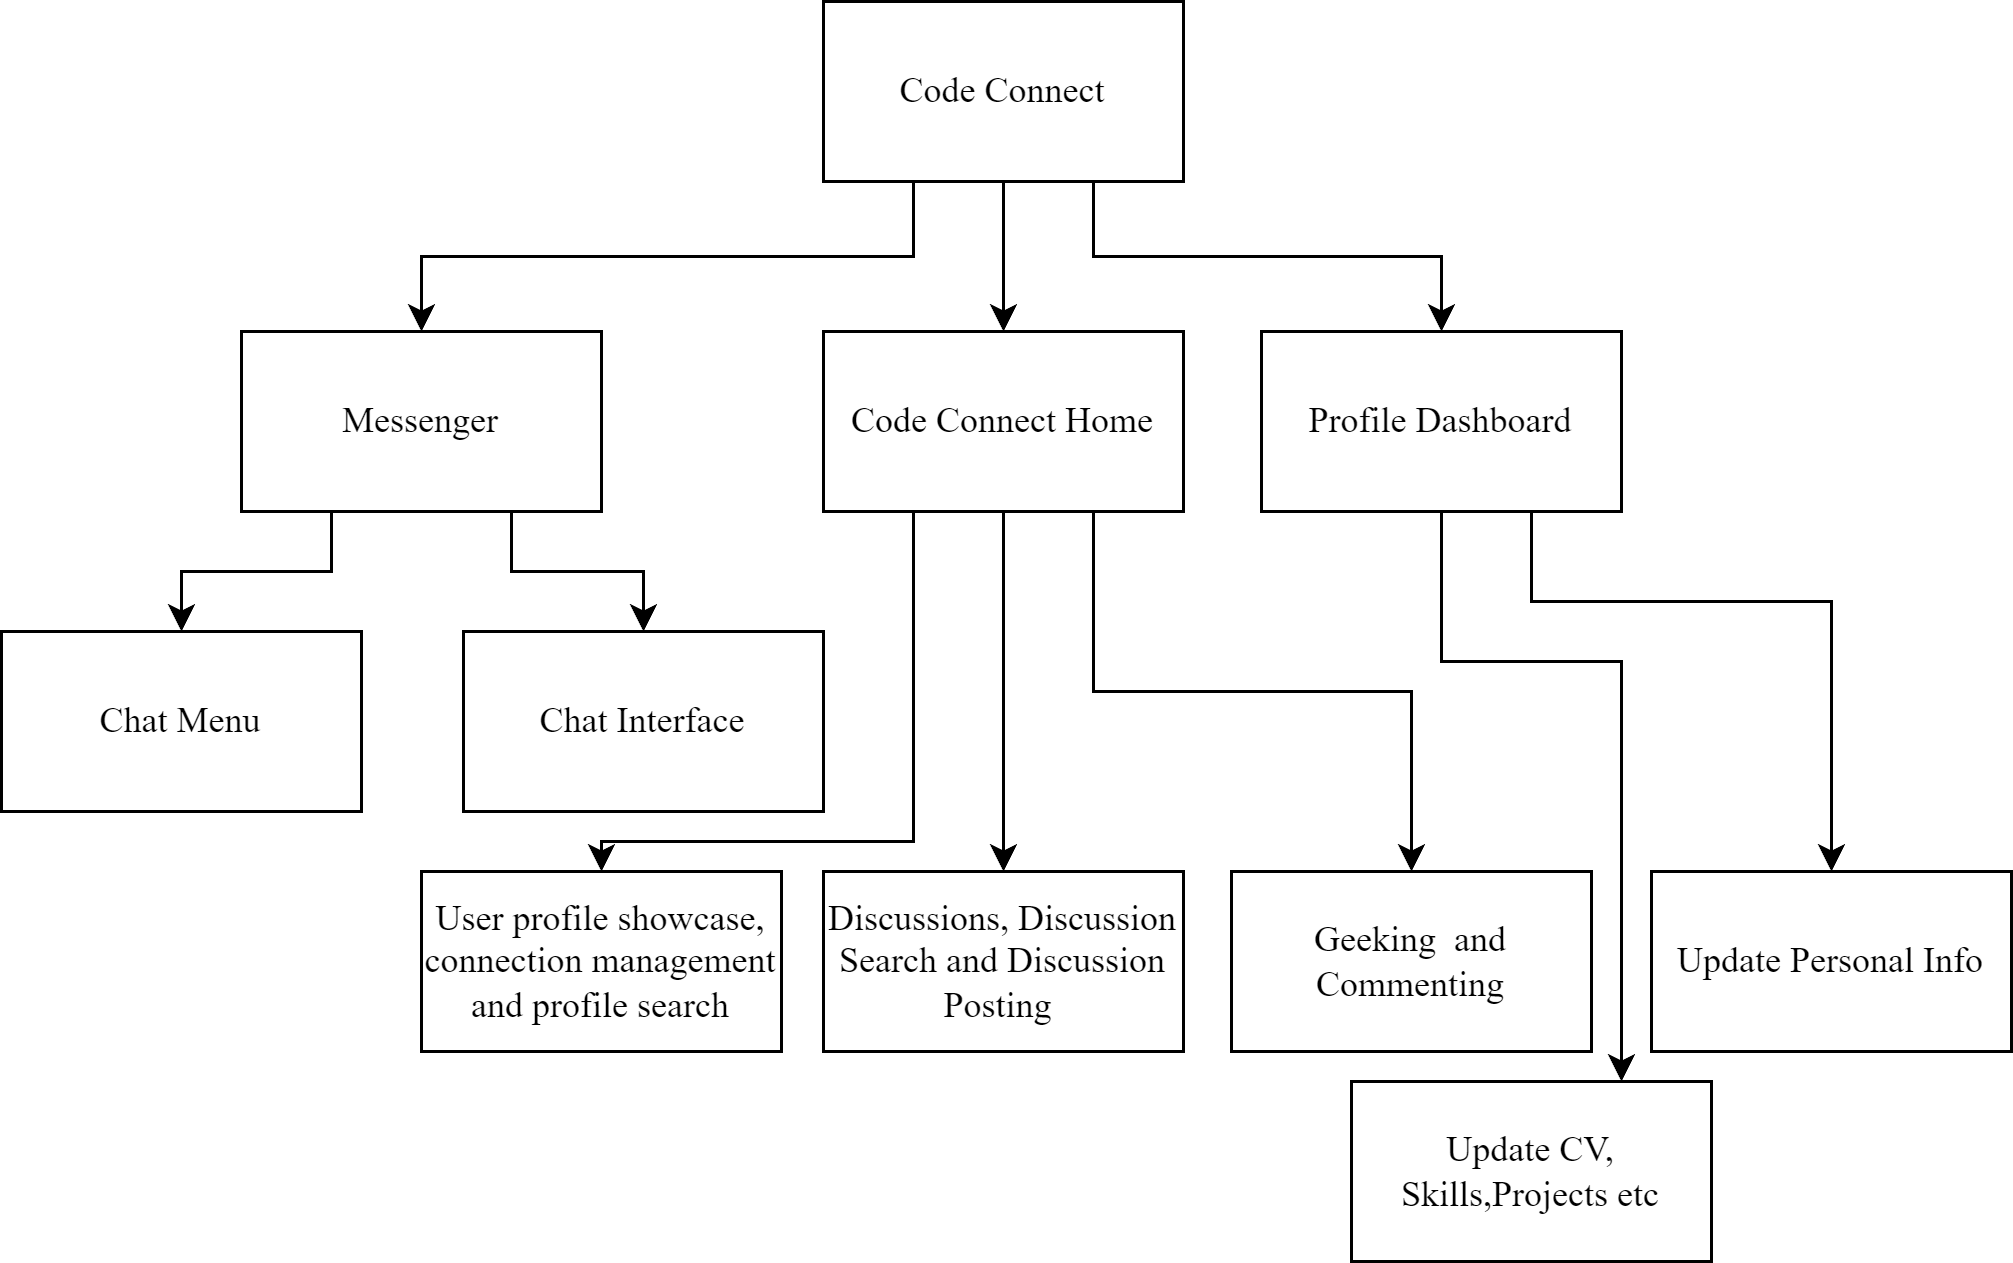
\includegraphics[height = 8cm]{Diagrams/Main_Block.png}
    \caption{Main Architecture of System}
\end{figure}
\newpage
\subsection{Data Modelling(ER-Diagram)}
ER Diagram is mainly used to design database schema. With the help of below er diagram we can easily design database in SQL.
\begin{figure}[H]
    \rotatebox{90}{
    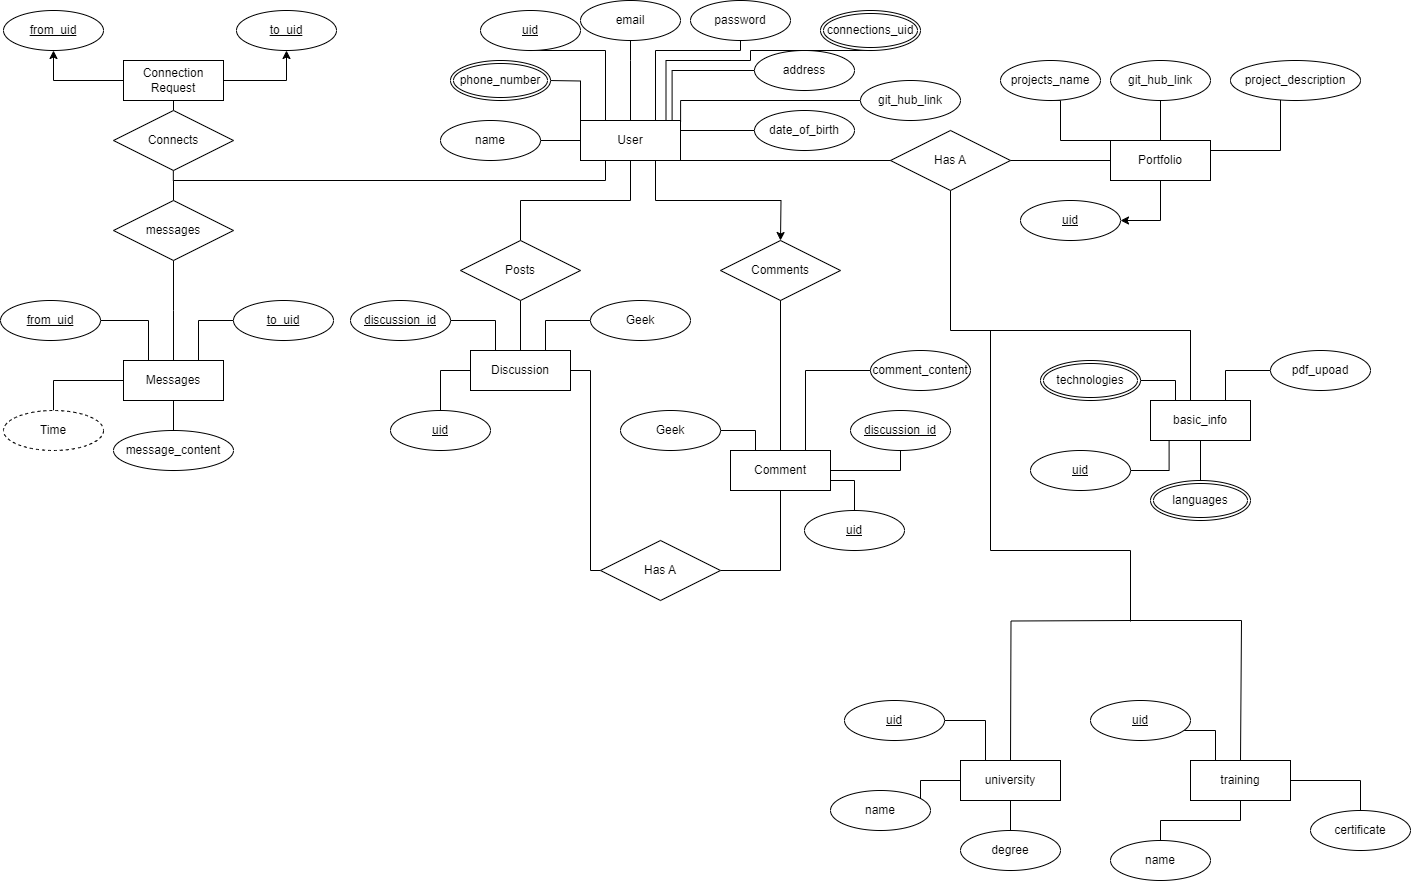
\includegraphics[height = 12cm]{Diagrams/er.drawio.png}}
    \caption{ER Diagram of System Data}
\end{figure}
\newpage
\subsection{Activity Diagram}
An activity diagram visually presents a series of actions or flow of control in a system similar to a flowchart or a data flow diagram. This diagram showed how our program flow goes on.
\begin{figure}[H]
   \centering
    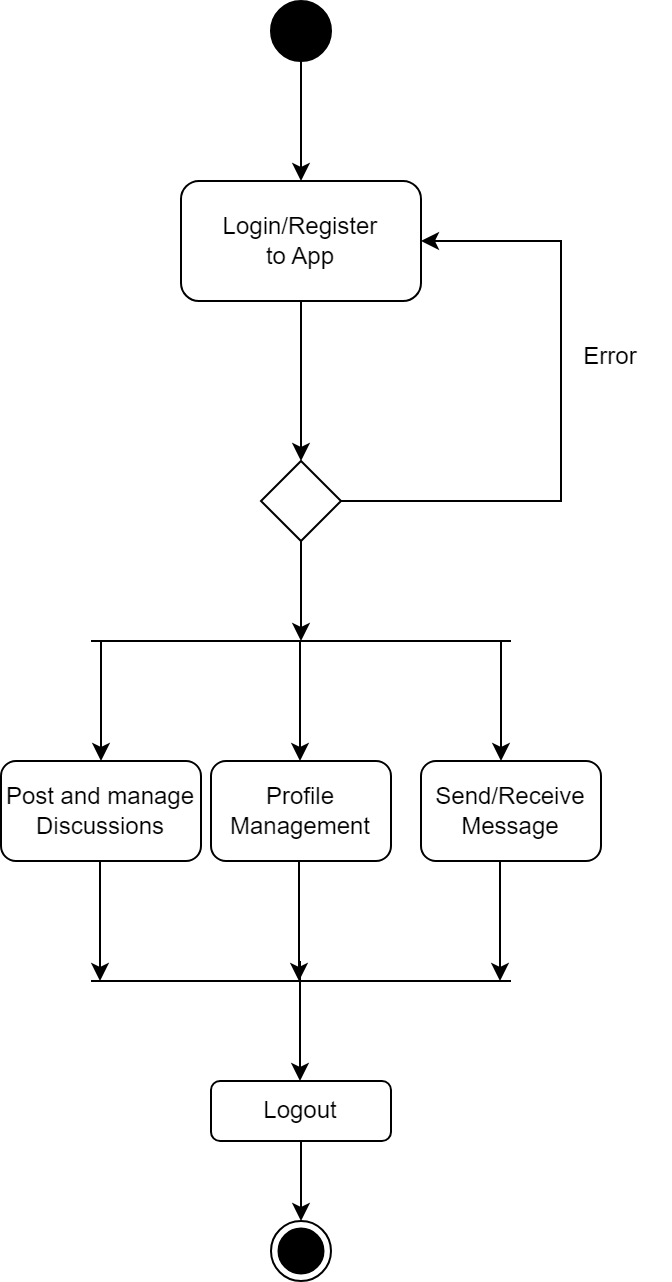
\includegraphics[height = 15cm]{Diagrams/Activity.drawio.png}
    \caption{Activity Diagram}
\end{figure}
\newpage
\subsection{DFD}
DFD or Data Flow Diagram is mainly used to show how data are being flowed in and out of our system. There are 3 levels of DFD i.e Context Level(Level 0),Level 1 and Level 2
\begin{figure}[H]
    \centering
    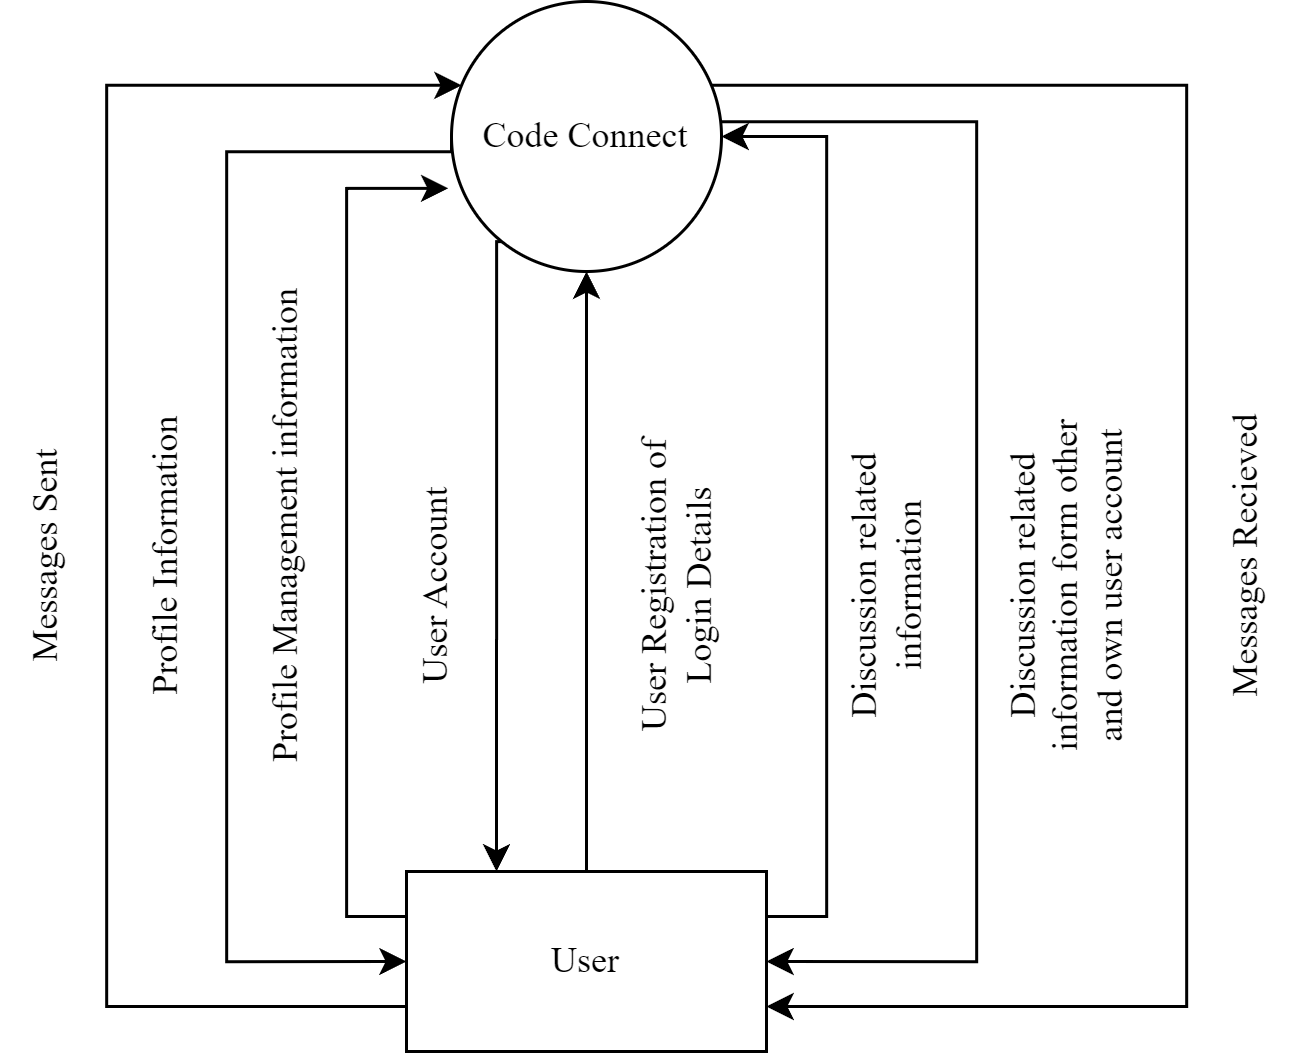
\includegraphics[height = 8cm]{Diagrams/DFD.drawio.png}
    \caption{Data Flow Diagram (Context Level)}
\end{figure}
\newpage
\subsection{Use Case Diagram}
A use case diagram, part of UML, visually represents interactions between actors and a system. Actors are external entities, while use cases depict specific functionalities. Relationships, such as association, generalization, include, and extend, illustrate connections between actors and use cases. The diagram helps in understanding system behavior, requirements, and scope.
\begin{figure}[H]
    \rotatebox{90}{
    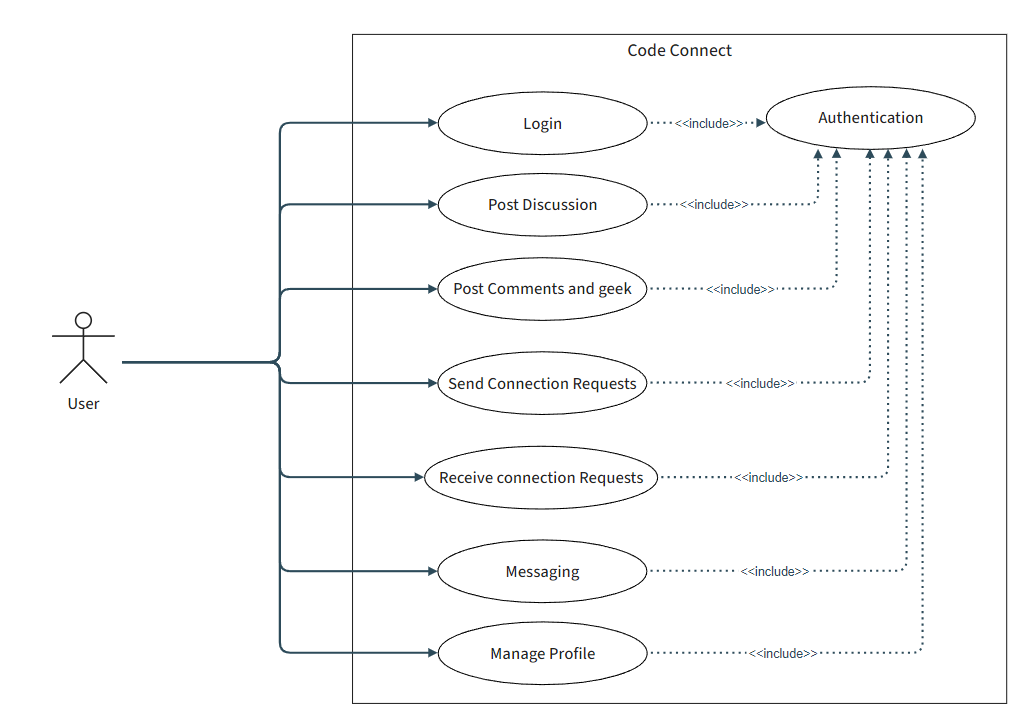
\includegraphics[height = 12cm]{Diagrams/use_case.png}}
    \caption{Use Case Diagram}
\end{figure}

\chapter{IMPLEMENTATION AND TESTING}
\section{Implementation}
"Code Connect" is a delightful online space where programmers come together to share ideas and experiences. Using tools like HTML, CSS, and JavaScript, we've built a website that's easy to use and fun to explore. Behind the scenes, PHP and MySQL work like magic to handle all the information. With AJAX and JQuery, everything feels smooth and interactive, just like chatting with friends. It's not just about technology – it's about people connecting and learning from each other. Just like baking a tasty treat, we've mixed all these ingredients to create something special that everyone can enjoy.


% (20\% of Report Length)

% a. Showcase the output at various intermediate stages of the project pipeline

% b. Use proper data visualizing techniques to present the output

% c. Figures and tables must be accompanied by an explanation
\section{Tools Used}
\subsection{Git}
Git is a fundamental version control system for software development, efficiently managing changes through commits. It fosters collaboration via branches and seamless merging, acts as a backup mechanism, and encourages code reviews for quality improvement. Git's popularity in open-source projects facilitates global collaboration, and its integration with CI/CD pipelines automates testing and deployment. In essence, Git empowers teams with version control, collaboration capabilities, and streamlined change management, enhancing project development.
\subsection{Figma}
Figma, a cloud-based design and prototyping tool, is renowned for its real-time collaboration, allowing multiple users to work together seamlessly. It offers robust design features like vector editing, typography controls, and color management. Designers can create interactive prototypes with clickable elements and animations, simulating user interactions effectively. Figma promotes design consistency through component libraries and simplifies handoff with easy sharing of specs and assets. It enhances stakeholder engagement, supports user testing, and integrates with various tools, making it a versatile choice for teams focused on delivering compelling digital experiences.
\subsection{GitHub}
GitHub is a pivotal web-based platform for software development, utilizing Git for version control and centralized code hosting. Multiple developers collaborate simultaneously using branches and pull requests for code review. It boasts an integrated issue tracker, wikis, and documentation for enhanced accessibility. GitHub seamlessly integrates with CI/CD tools and fosters open-source community participation. Security measures include vulnerability scanning and permissions management. In summary, GitHub serves as a collaborative hub for version control, code management, issue tracking, and community involvement, enabling efficient software development.
\subsection{HTML, CSS and JS}
\begin{itemize}
    \item \textbf{HTML (Hypertext Markup Language)}: HTML is the foundational language used to create the structure of web content. It uses a system of tags to define elements like headings, paragraphs, links, images, and more. These tags give structure to web pages, organizing content into a meaningful layout. HTML provides the framework for displaying information and forming the basis for user interaction on the web.

    \item \textbf{CSS (Cascading Style Sheets)}: CSS is a styling language that complements HTML by controlling the visual presentation of web content. It allows developers to define colors, fonts, margins, borders, and other design aspects of HTML elements. By separating content from presentation, CSS enables consistent styling across web pages and enhances user experience through improved aesthetics and readability.

    \item \textbf{JavaScript (JS)}: JavaScript is a versatile scripting language used to add interactivity and dynamic behavior to web pages. It enables developers to create responsive features such as form validation, animations, pop-ups, and real-time updates. JS executes directly in the browser, allowing users to interact with web content without requiring page reloads. It's a crucial component for creating engaging and interactive web experiences.

\end{itemize}
\subsection{MySQL}
MySQL, an open-source relational database management system (RDBMS), excels in organizing structured data for various applications. It's proficient in SQL (Structured Query Language), allowing effortless database creation, data relationships, and advanced queries. MySQL ensures data integrity, speedy retrieval through indexing, and reliable transaction management. It supports collaborative data work with security. Whether for small projects or enterprise endeavors, MySQL's adaptability, strong community, and compatibility make it the go-to choice for data management and robust application development.
\subsection{PHP}
In the realm of web development, PHP stands out as a powerful scripting language, capable of creating dynamic and interactive websites. Integrated seamlessly with HTML, PHP empowers websites to process forms, communicate with databases, and deliver content that adapts to user actions. Its open-source nature fosters a collaborative community of developers. For both beginners and experts, PHP is an invaluable tool, enhancing web projects with its functionality and innovation. It serves as a cornerstone in modern web development, essential for crafting standout websites in the digital landscape.
\section{Modules Used}
\subsection{AJAX}
In the dynamic world of web development, AJAX (Asynchronous JavaScript and XML) stands out as a transformative technique. It combines JavaScript and server communication to enable seamless, asynchronous data exchange. Unlike traditional methods, AJAX allows developers to update specific sections of a web page without full page reloads, enhancing user experience. AJAX's compatibility with data formats like XML and JSON enables efficient data transmission, facilitating real-time updates and interactive web applications. This technique elevates user engagement and pushes modern web development into a new era of possibilities.
\subsection{JQuery}
In the realm of web development, jQuery emerges as a transformative force, simplifying complex tasks and enhancing user interaction. This fast, compact JavaScript library streamlines DOM manipulation, making it effortless to select, modify, and animate HTML elements. jQuery's user-friendly syntax and built-in functions mitigate cross-browser compatibility issues, ensuring seamless development across platforms. Its extensive plugin ecosystem adds pre-built functionalities to projects, abstracting complex JavaScript operations into concise commands for cleaner code and faster development. With capabilities in event handling, animations, and AJAX requests, jQuery accelerates the creation of engaging, feature-rich web applications.
\subsection{MySqli Connect}
In the world of web development and database connectivity, the mysqli\_connect function stands as a fundamental tool worth exploring. Within the PHP programming language, it plays a pivotal role in establishing secure links between web applications and MySQL databases. By providing essential parameters like host, username, password, and database name, developers can effortlessly create a communication channel with MySQL servers. This function is crucial for enabling dynamic and interactive web applications, serving as the foundational bridge for data-driven features. mysqli\_connect significantly contributes to the efficiency and responsiveness of modern database-driven web development, making it an essential component.
\subsection{Google Fonts}
In the realm of web design and typography, Google Fonts emerges as a transformative tool. Its extensive collection of meticulously curated fonts offers designers an array of creative possibilities. Beyond aesthetics, Google Fonts prioritizes user experience, promoting accessible and visually appealing text choices. The user-friendly interface and seamless integration make font selection and embedding effortless. Furthermore, it optimizes performance, ensuring that design enhancements don't hinder website speed. My exploration of Google Fonts highlights its value in enhancing both the aesthetics and accessibility of web content significantly.
\subsection{Font Awesome }
In the world of web design and user interface enhancement, Font Awesome stands out as a remarkable tool. Its extensive icon library, spanning diverse categories, simplifies icon integration into web projects. Font Awesome not only adds visual appeal but also enhances functionality. Using CSS classes for seamless icon incorporation and customization options for size, color, and style, it empowers designers for creative expression. Its compatibility with various frameworks and platforms makes it versatile for all developers. Font Awesome significantly elevates user experiences by adding depth and meaning to digital interfaces, making it an essential asset in crafting captivating and user-centric web applications.
\subsection{Bootstrap}
We have used small portion of bootstrap for quick development of profile dashboard. Bootstrap is a widely-used front-end framework that simplifies web development by providing a collection of pre-designed HTML, CSS, and JavaScript components. With its responsive design, ready-made elements, and customization options, Bootstrap enables developers to create mobile-friendly and visually appealing websites and web applications with ease.
% \subsection{Implementation Details of Modules}
% \section{Testing}
% \subsection{Test Cases for Unit Testing}
% \subsection{Test Cases for System Testing}
\section{Testing}
\subsection{Unit Testing}
Unit testing is a software testing technique where individual units or components of a software application are tested in isolation to ensure that they function correctly. These units can be functions, methods, classes, or even small modules. Unit testing aims to verify that each unit performs as expected, providing developers with confidence that their code works as intended and catches bugs early in the development process.
\\
\textbf{Authenication Unit}\\
Here testing different test cases of authentication system in Code Connect is performed as required:\\
\begin{table}[H]
    \caption{Authenication Unit Testing}
        \label{}
    \begin{tabular}{|p{0.3in}|p{1.2in}|p{1.2in}|p{1.2in}|p{1in}|}
        \hline
        Tests & Test Cases & Input & Expected Output & Actual Output \\
        \hline
            1 & Incorrect Password& Email:\url{test@gmail.com} Password:1234& Incorrect Password& Incorrect Password \\
            \hline
            2 & Incorrect Confirm Password in SignUp & Email:\url{test@gmail.com}
            Password:12345679
            Password:12345678 & Enter Same Password & Enter Same Password \\
            \hline
            3 & Correct Credentials In Login & Email:\url{test@gmail.com}
            Password:12345679 & Redirects to homepage & Redirects to homepage \\
            \hline
\end{tabular}
\end{table}

\textbf{Launch Application when user is not logged-in}\\
\begin{table}[H]
    \caption{Launch Application when user is not logged-in Testing}
        \label{}
    \begin{tabular}{|p{0.3in}|p{1.2in}|p{1.2in}|p{1.2in}|p{1in}|}
        \hline
        Tests & Test Cases & Input &Expected Output & Actual Output \\
        \hline
            1 & Launch application& \url{http://localhost/codeconnect/login/}& Log-In page& Log-In page \\
            \hline
\end{tabular}
\end{table}

\textbf{Launch Application when user is already logged-in}\\
\begin{table}[H]
    \caption{Launch Application when user is already logged-in Testing}
        \label{}
    \begin{tabular}{|p{0.3in}|p{1.2in}|p{1.2in}|p{1.2in}|p{1in}|}
        \hline
        Tests & Test Cases & Input &Expected Output & Actual Output \\
        \hline
            1 & Launch application& \url{http://localhost/codeconnect/home/}& CodeConnect Home page& CodeConnect Home page \\
            \hline
\end{tabular}
\end{table}

\textbf{Code Connect Messenger}\\
\begin{table}[H]
    \caption{Code Connect Messenger Testing}
        \label{}
    \begin{tabular}{|p{0.3in}|p{1.2in}|p{1.2in}|p{1.2in}|p{1in}|}
        \hline
        Tests & Test Cases & Input &Expected Output & Actual Output \\
        \hline
            1 & Code Connect Messenger& \url{http://localhost/codeconnect/messenger/}& Code Connect Messenger&  Code Connect Messenger \\
            \hline
\end{tabular}
\end{table}

\textbf{Send Message}\\
\begin{table}[H]
    \caption{Code Connect Send Message to other user Testing}
        \label{}
    \begin{tabular}{|p{0.3in}|p{1.2in}|p{1.2in}|p{1.2in}|p{1in}|}
        \hline
        Tests & Test Cases & Input &Expected Output & Actual Output \\
        \hline
            1 & Send message& click on messenger button and click on other user that is located at the left side to start a conversations& Sends message to that particular user& Sends message to that particular user \\
            \hline
\end{tabular}
\end{table}

\newpage
\textbf{Receive Message}\\
\begin{table}[H]
    \caption{Code Connect Receive Message from other user Testing}
        \label{}
    \begin{tabular}{|p{0.3in}|p{1.2in}|p{1.2in}|p{1.2in}|p{1in}|}
        \hline
        Tests & Test Cases & Input &Expected Output & Actual Output \\
        \hline
            1 & Receive message& click on messenger button and click on other user that is located at the left side to see the conversation& Display the conversation with that particular user& Display the conversation with that particular user\\
            \hline
\end{tabular}
\end{table}

\textbf{Code Connect Search User}\\
\begin{table}[H]
    \caption{Code Connect Search User Testing}
        \label{}
    \begin{tabular}{|p{0.3in}|p{1.2in}|p{1.2in}|p{1.2in}|p{1in}|}
        \hline
        Tests & Test Cases & Input &Expected Output & Actual Output \\
        \hline
            1 & Code Connect Search User& Si& Name of user starting from "Si"& Sirjan Shrestha \\
            \hline
\end{tabular}
\end{table}

\textbf{Code Connect Search Posts}\\
\begin{table}[H]
    \caption{Code Connect Search Posts Testing}
        \label{}
    \begin{tabular}{|p{0.3in}|p{1.2in}|p{1.2in}|p{1.2in}|p{1in}|}
        \hline
        Tests & Test Cases & Input &Expected Output & Actual Output \\
        \hline
            1 & Code Connect Search Posts& python& Posts that have content of python& python posts \\
            \hline
\end{tabular}
\end{table}

\newpage
\textbf{Show posts of friends only}\\
\begin{table}[H]
    \caption{Show posts of friends only Testing}
        \label{}
    \begin{tabular}{|p{0.3in}|p{1.2in}|p{1.2in}|p{1.2in}|p{1in}|}
        \hline
        Tests & Test Cases & Input &Expected Output & Actual Output \\
        \hline
            1 &Show posts of friends only& Click on the Friends Only button located at post section& Shows Posts of Friends only& Shows posts of friends only \\
            \hline
\end{tabular}
\end{table}

\textbf{Show all posts}\\
\begin{table}[H]
    \caption{Show all posts Testing}
        \label{}
    \begin{tabular}{|p{0.3in}|p{1.2in}|p{1.2in}|p{1.2in}|p{1in}|}
        \hline
        Tests & Test Cases & Input &Expected Output & Actual Output \\
        \hline
            1 &Show all posts& Click on the Public button located at post section& Shows Posts of all users& Shows posts of all users \\
            \hline
\end{tabular}
\end{table}

\textbf{Make Posts}\\
\begin{table}[H]
    \caption{Make Posts Testing}
        \label{}
    \begin{tabular}{|p{0.3in}|p{1.2in}|p{1.2in}|p{1.2in}|p{1in}|}
        \hline
        Tests & Test Cases & Input &Expected Output & Actual Output \\
        \hline
            1 & Make posts& Click on post button& Open Post Menu& Opens Posts Menu \\
            \hline
\end{tabular}
\end{table}

\newpage
\textbf{Making Post including content on both Post and Coding section}\\
\begin{table}[H]
    \caption{Making Post including content on both Post and Coding section Testing}
        \label{}
    \begin{tabular}{|p{0.3in}|p{1.2in}|p{1.2in}|p{1.2in}|p{1in}|}
        \hline
        Tests & Test Cases & Input &Expected Output & Actual Output \\
        \hline
            1 & Making Post including content on both Post and Coding section& Post section:coding in C Code section: printf("Hello World");& post including both of the section& made post including both of the section\\
            \hline
\end{tabular}
\end{table}

\textbf{Delete Posts}\\
\begin{table}[H]
    \caption{Delete Posts Testing}
        \label{}
    \begin{tabular}{|p{0.3in}|p{1.2in}|p{1.2in}|p{1.2in}|p{1in}|}
        \hline
        Tests & Test Cases & Input &Expected Output & Actual Output \\
        \hline
            1 & Delete posts&After visiting self profile, Click on delete post button& Deletion of that particular post& Delets the post \\
            \hline
\end{tabular}
\end{table}

\textbf{Geeking on post}\\
\begin{table}[H]
    \caption{Geeking on post Testing}
        \label{}
    \begin{tabular}{|p{0.3in}|p{1.2in}|p{1.2in}|p{1.2in}|p{1in}|}
        \hline
        Tests & Test Cases & Input &Expected Output & Actual Output \\
        \hline
            1 & Geeking on Posts & Press Geek button& count Geek of users on post & counts Geek of users on post \\
            \hline
\end{tabular}
\end{table}

\newpage
\textbf{Un-Geeking on post}\\
\begin{table}[H]
    \caption{Un-Geeking on post Testing}
        \label{}
    \begin{tabular}{|p{0.3in}|p{1.2in}|p{1.2in}|p{1.2in}|p{1in}|}
        \hline
        Tests & Test Cases & Input &Expected Output & Actual Output \\
        \hline
            1 & Un-Geeking on Posts & Press Geek button again & Deletion of geek count of that user &Delets the geek count of that user \\
            \hline
\end{tabular}
\end{table}

\textbf{Commenting on post}\\
\begin{table}[H]
    \caption{Commenting on post Testing}
        \label{}
    \begin{tabular}{|p{0.3in}|p{1.2in}|p{1.2in}|p{1.2in}|p{1in}|}
        \hline
        Tests & Test Cases & Input &Expected Output & Actual Output \\
        \hline
            1 &Commenting on post & Press comment button and write comment & comment of users on that particular post & comment of users on that particular post \\
            \hline
\end{tabular}
\end{table}

\textbf{Deleting Comment on post}\\
\begin{table}[H]
    \caption{Deleting Comment on post Testing}
        \label{}
    \begin{tabular}{|p{0.3in}|p{1.2in}|p{1.2in}|p{1.2in}|p{1in}|}
        \hline
        Tests & Test Cases & Input &Expected Output & Actual Output \\
        \hline
            1 &Deleting Comment on post & Press delete button & Deletion of comment of that user& Delets the comment of that user \\
            \hline
\end{tabular}
\end{table}

\newpage
\textbf{Saving post}\\
\begin{table}[H]
    \caption{Saving post Testing}
        \label{}
    \begin{tabular}{|p{0.3in}|p{1.2in}|p{1.2in}|p{1.2in}|p{1in}|}
        \hline
        Tests & Test Cases & Input &Expected Output & Actual Output \\
        \hline
            1 &Saving post & Press save button located at right side of post & Save the posts & Saves that post \\
            \hline
\end{tabular}
\end{table}

\textbf{Un-Saving post}\\
\begin{table}[H]
    \caption{Un-Saving post Testing}
        \label{}
    \begin{tabular}{|p{0.3in}|p{1.2in}|p{1.2in}|p{1.2in}|p{1in}|}
        \hline
        Tests & Test Cases & Input &Expected Output & Actual Output \\
        \hline
            1 &Un-Saving post & Press save button again that is located at right side of post & Removes the saved post &  Removes the saved post  \\
            \hline
\end{tabular}
\end{table}

\textbf{Profile Dashboard}\\
\begin{table}[H]
    \caption{Profile Dashboard Testing}
        \label{}
    \begin{tabular}{|p{0.3in}|p{1.2in}|p{1.2in}|p{1.2in}|p{1in}|}
        \hline
        Tests & Test Cases & Input &Expected Output & Actual Output \\
        \hline
            1 &Visiting Profile Dashboard & Press on Profile Dashboard button after visiting self-profile &Show the profile Dashboard menu &Opens the profile Dashboard menu  \\
            \hline
\end{tabular}
\end{table}

\newpage
\textbf{Update Basic Account Details}\\
\begin{table}[H]
    \caption{Update Basic Account Details Testing}
        \label{}
    \begin{tabular}{|p{0.3in}|p{1.2in}|p{1.2in}|p{1.2in}|p{1in}|}
        \hline
        Tests & Test Cases & Input &Expected Output & Actual Output \\
        \hline
            1 &Update Basic Account Details & Press on Update Basic Account Details button after visiting profile dashboard &Opens the form that helps the user to update their basic informations  &Opens the form that helps the user to update their basic informations  \\
            \hline
\end{tabular}
\end{table}

\textbf{Update Projects}\\
\begin{table}[H]
    \caption{Update Projects Testing}
        \label{}
    \begin{tabular}{|p{0.3in}|p{1.2in}|p{1.2in}|p{1.2in}|p{1in}|}
        \hline
        Tests & Test Cases & Input &Expected Output & Actual Output \\
        \hline
            1 &Update Projects & Press on Update Projects button after visiting profile dashboard &Opens the form that helps the user to update their Projects  &Opens the form that helps the user to update their Projects  \\
            \hline
\end{tabular}
\end{table}

\textbf{Update Certification}\\
\begin{table}[H]
    \caption{Update Certification Testing}
        \label{}
    \begin{tabular}{|p{0.3in}|p{1.2in}|p{1.2in}|p{1.2in}|p{1in}|}
        \hline
        Tests & Test Cases & Input &Expected Output & Actual Output \\
        \hline
            1 &Update Certification & Press on Update Certification button after visiting profile dashboard &Opens the form that helps the user to update their Certifications  &Opens the form that helps the user to update their Certifications  \\
            \hline
\end{tabular}
\end{table}

\newpage
\textbf{Update Skills}\\
\begin{table}[H]
    \caption{Update Skills Testing}
        \label{}
    \begin{tabular}{|p{0.3in}|p{1.2in}|p{1.2in}|p{1.2in}|p{1in}|}
        \hline
        Tests & Test Cases & Input &Expected Output & Actual Output \\
        \hline
            1 &Update Skills & Press on Update skills button after visiting profile dashboard &Opens the form that helps the user to update their skills  &Opens the form that helps the user to update their skills  \\
            \hline
\end{tabular}
\end{table}

\textbf{Update CV}\\
\begin{table}[H]
    \caption{Update CV Testing}
        \label{}
    \begin{tabular}{|p{0.3in}|p{1.2in}|p{1.2in}|p{1.2in}|p{1in}|}
        \hline
        Tests & Test Cases & Input &Expected Output & Actual Output \\
        \hline
            1 &Update CV & Press on Update CV button after visiting profile dashboard &Opens the form that helps the user to update their CV  &Opens the form that helps the user to update their CV  \\
            \hline
\end{tabular}
\end{table}

\textbf{Code Connect Notification}\\
\begin{table}[H]
    \caption{Code Connect Notification Testing}
        \label{}
    \begin{tabular}{|p{0.3in}|p{1.2in}|p{1.2in}|p{1.2in}|p{1in}|}
        \hline
        Tests & Test Cases & Input &Expected Output & Actual Output \\
        \hline
            1 &Notification & Press on Notifiation button that is located at nav-bar &Open Notification Pannel that shows all the necessary notification &Open Notification Pannel that shows all the necessary notification \\
            \hline
\end{tabular}
\end{table}

\textbf{Send connection request}\\
\begin{table}[H]
    \caption{Send connection request Testing}
        \label{}
    \begin{tabular}{|p{0.3in}|p{1.2in}|p{1.2in}|p{1.2in}|p{1in}|}
        \hline
        Tests & Test Cases & Input &Expected Output & Actual Output \\
        \hline
            1 &Send connection request & After visiting other user's profile, Press on connect button that is located at side bard  &Send connection request to that particular user &Sends connection request to that particular user and shows connection reuested \\
            \hline
\end{tabular}
\end{table}

\textbf{Accept connection request}\\
\begin{table}[H]
    \caption{Accept connection request Testing}
        \label{}
    \begin{tabular}{|p{0.3in}|p{1.2in}|p{1.2in}|p{1.2in}|p{1in}|}
        \hline
        Tests & Test Cases & Input &Expected Output & Actual Output \\
        \hline
            1 &Accept connection request & Click on Accept Request button &Accept connection request of that particular user &Accept connection request of that particular user and adds that user to the connection list \\
            \hline
\end{tabular}
\end{table}

\newpage
\textbf{User Log-Out}\\
\begin{table}[H]
    \caption{User Log-Out Testing}
        \label{}
    \begin{tabular}{|p{0.3in}|p{1.2in}|p{1.2in}|p{1.2in}|p{1in}|}
        \hline
        Tests & Test Cases & Input &Expected Output & Actual Output \\
        \hline
            1 &User Log-Out & Click on Log-Out button that is located at the nav-bar &Logs the user out of the system &Logs the user out of the system and redirect the user to Log-In page \\
            \hline
\end{tabular}
\end{table}
% \begin{figure}[ht]
%     \centering
%     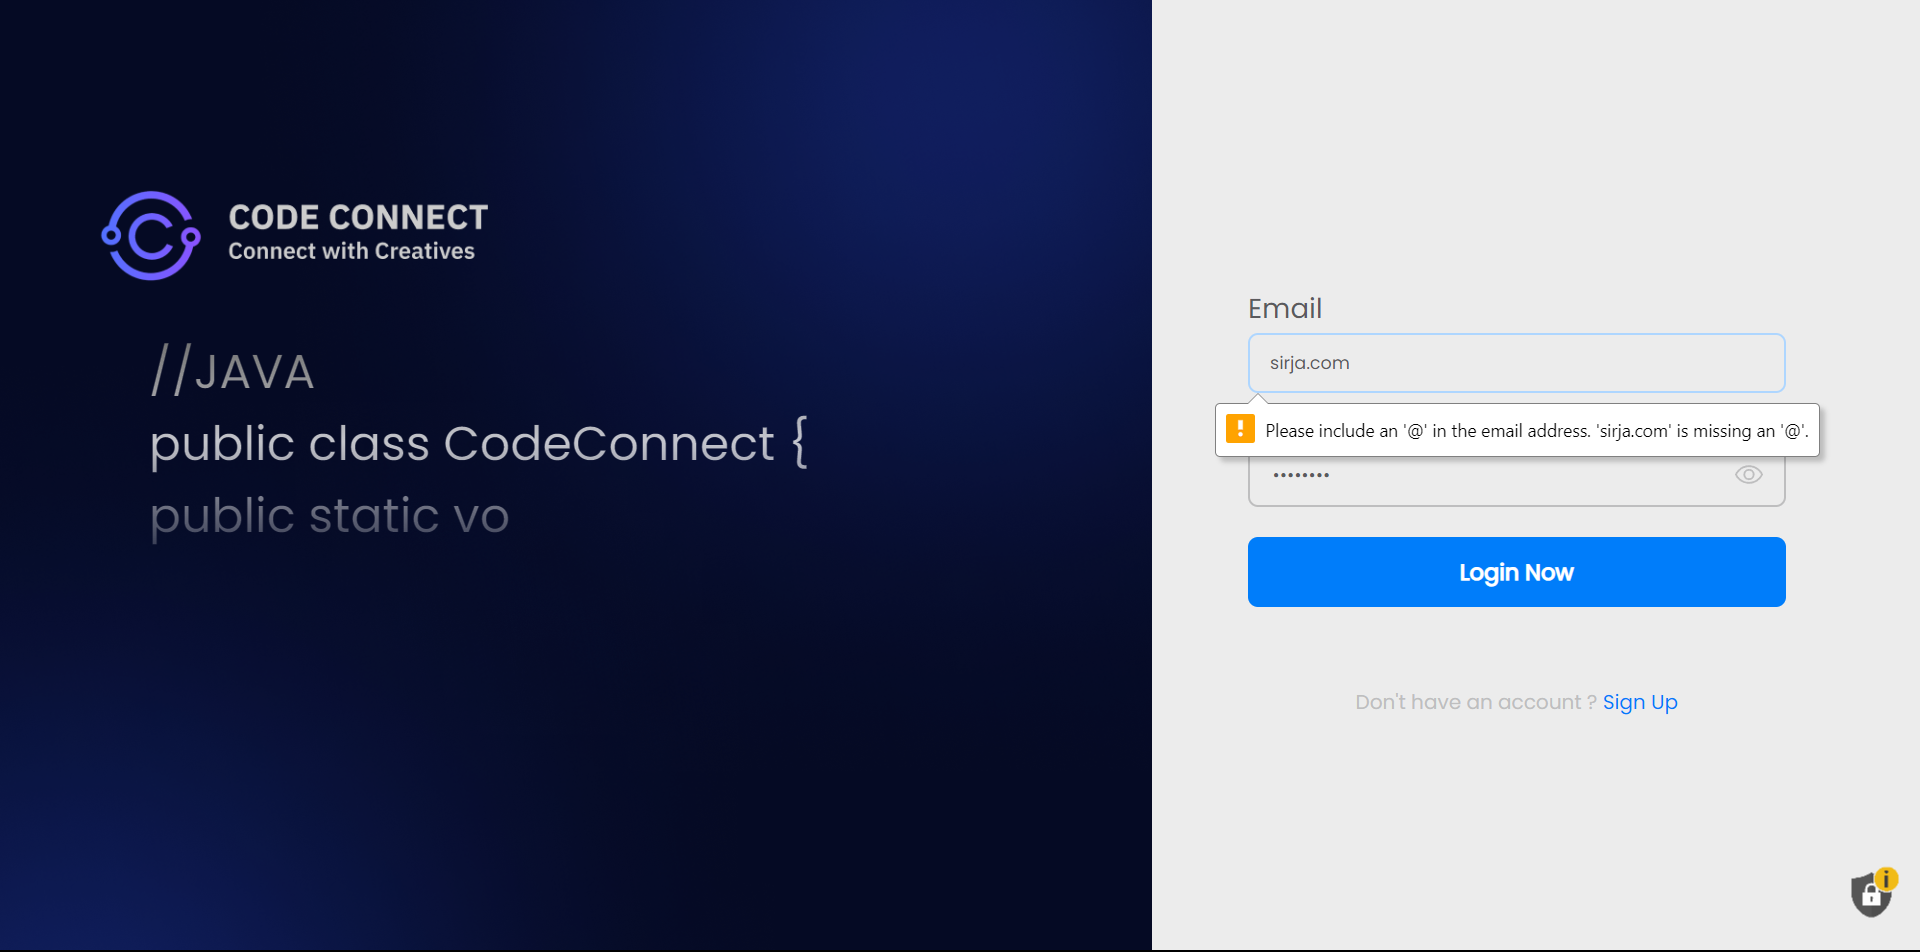
\includegraphics[width=1\textwidth]{4ImplementationAndTesting/screenshots/email-err-signin.png}
%     \caption{Incorrect email Format}
%     \label{fig: Incorrect email Format}

% \end{figure}
% \begin{figure}[ht]
%     \centering
%     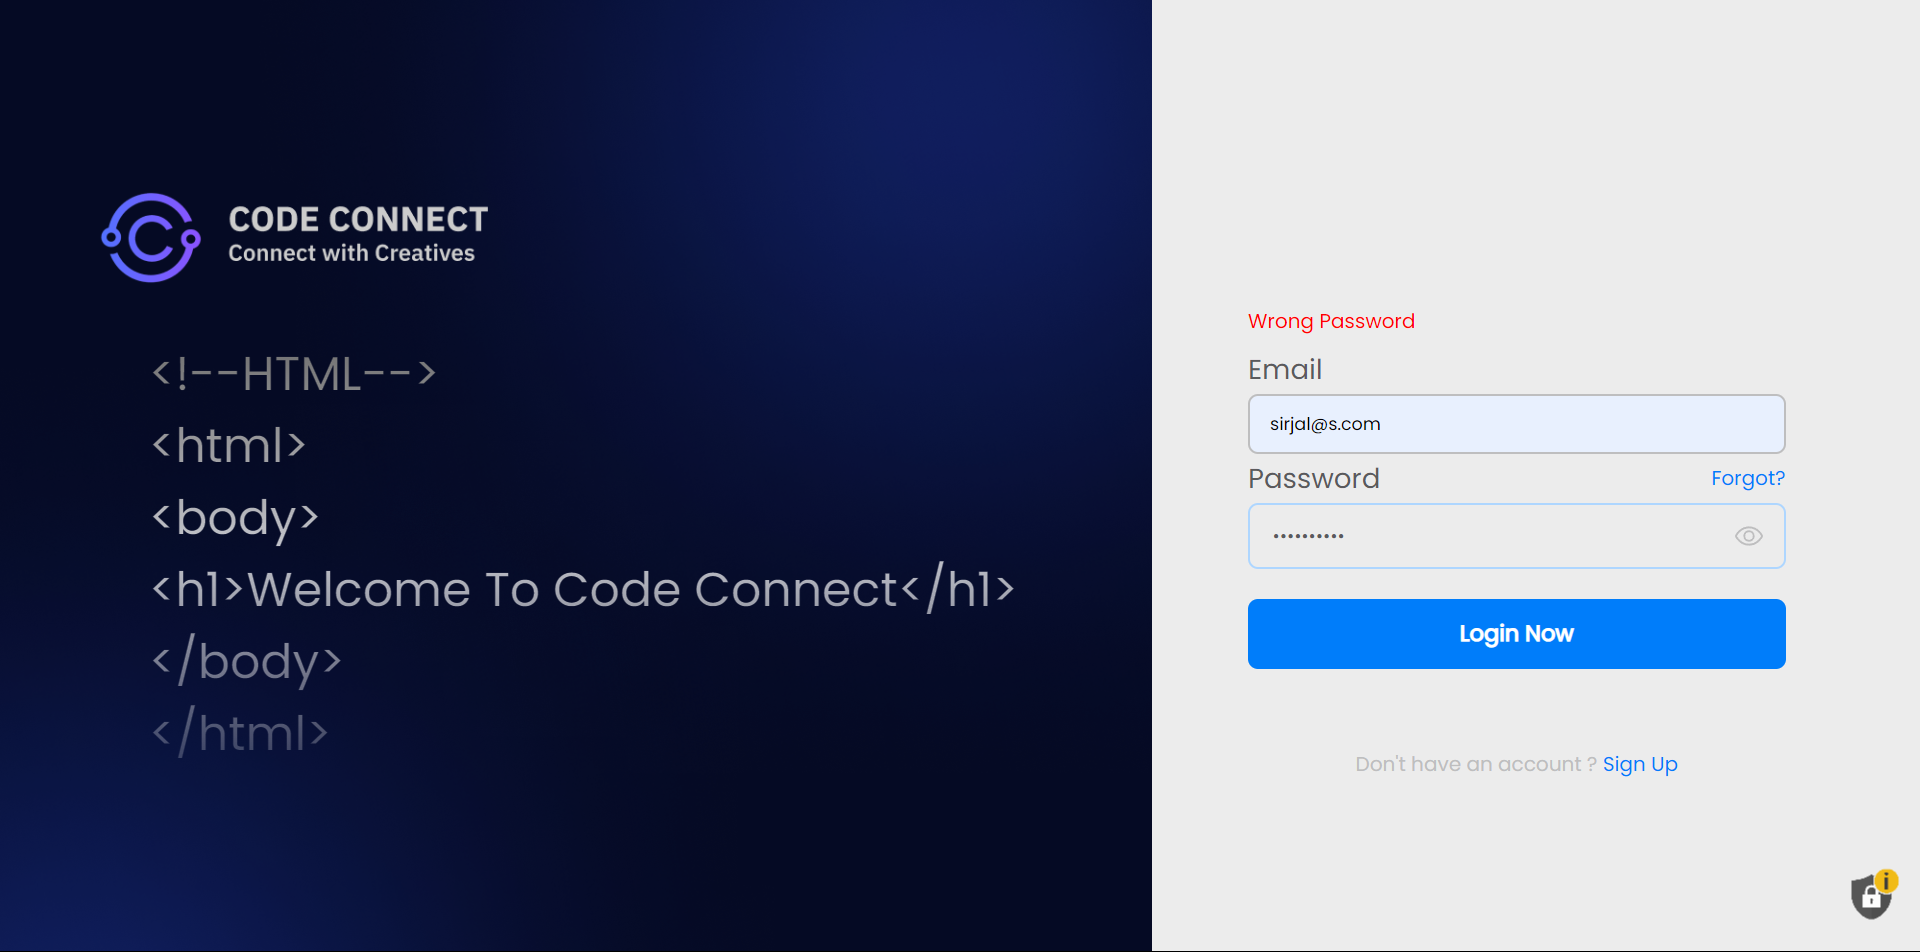
\includegraphics[width=1\textwidth]{4ImplementationAndTesting/screenshots/signin-pass-err.png}
%     \caption{Incorrect Password}
%     \label{fig: Incorrect Password}
% \end{figure}
% \begin{figure}[ht]
%     \centering
%     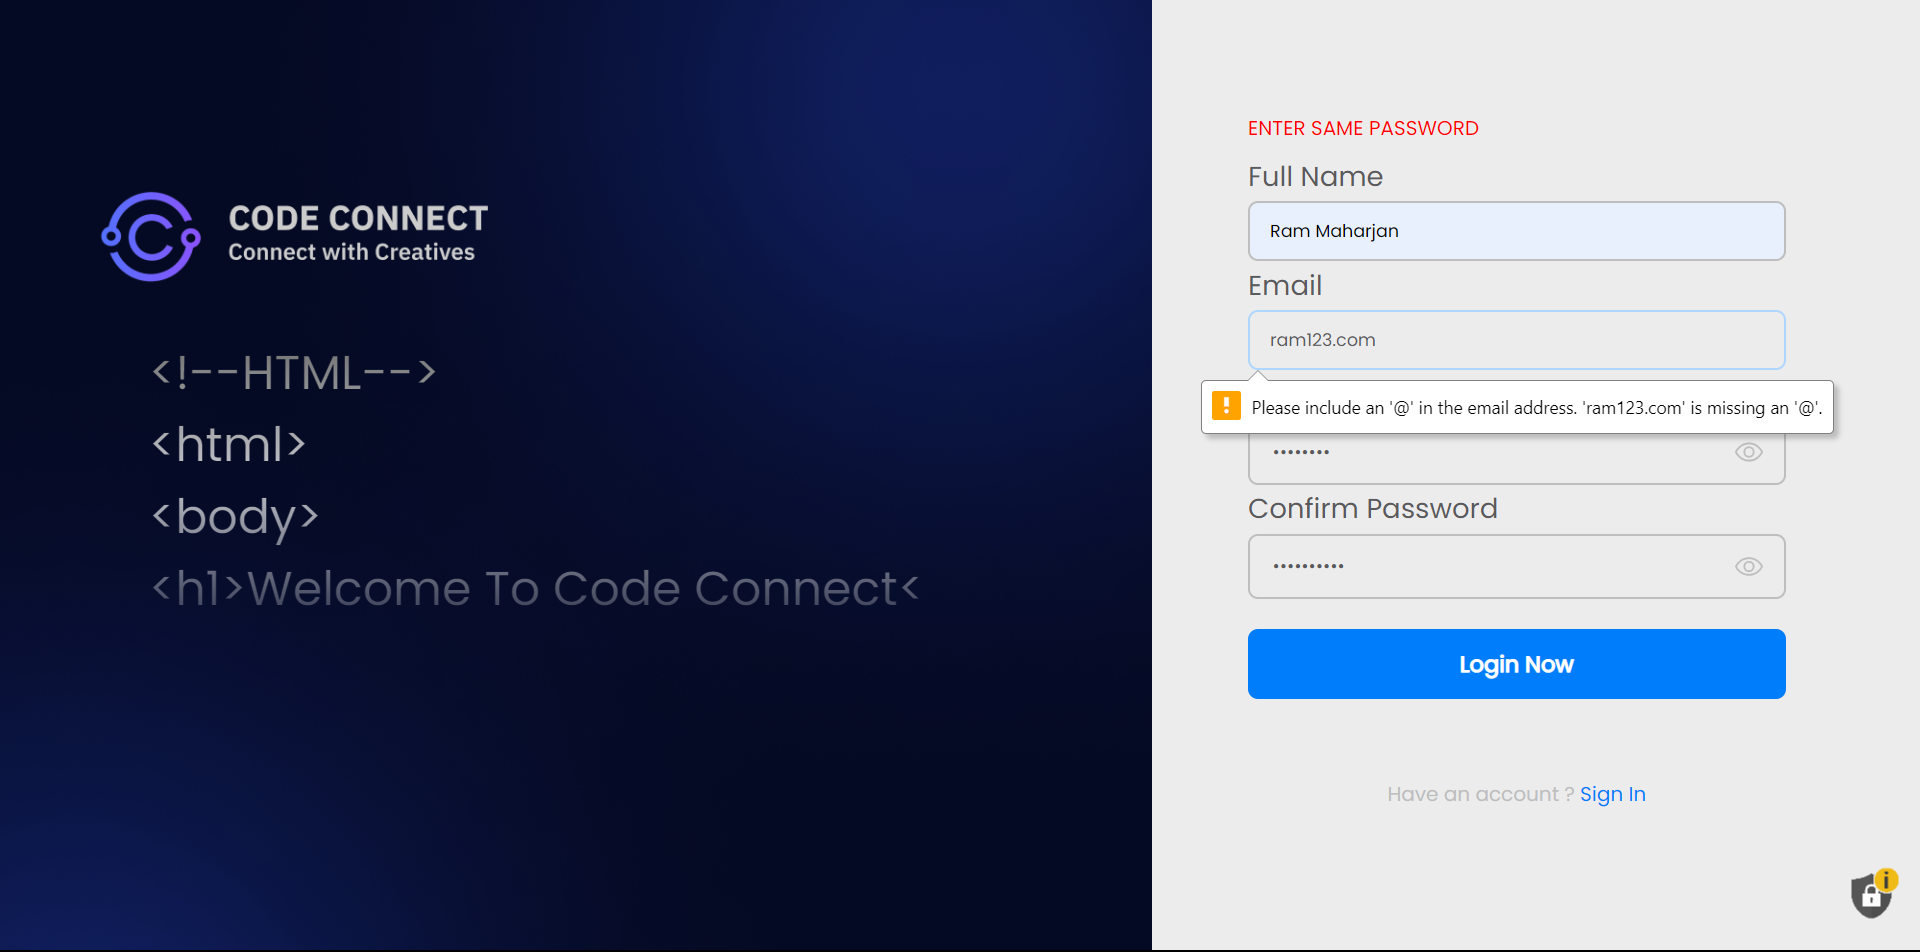
\includegraphics[width=1\textwidth]{4ImplementationAndTesting/screenshots/signup-same-pass.png}
%     \caption{Incorrect email Format In SignUp}
%     \label{fig: Incorrect email Format In SignUp}
% \end{figure}
% \begin{figure}[ht]
%     \centering
%     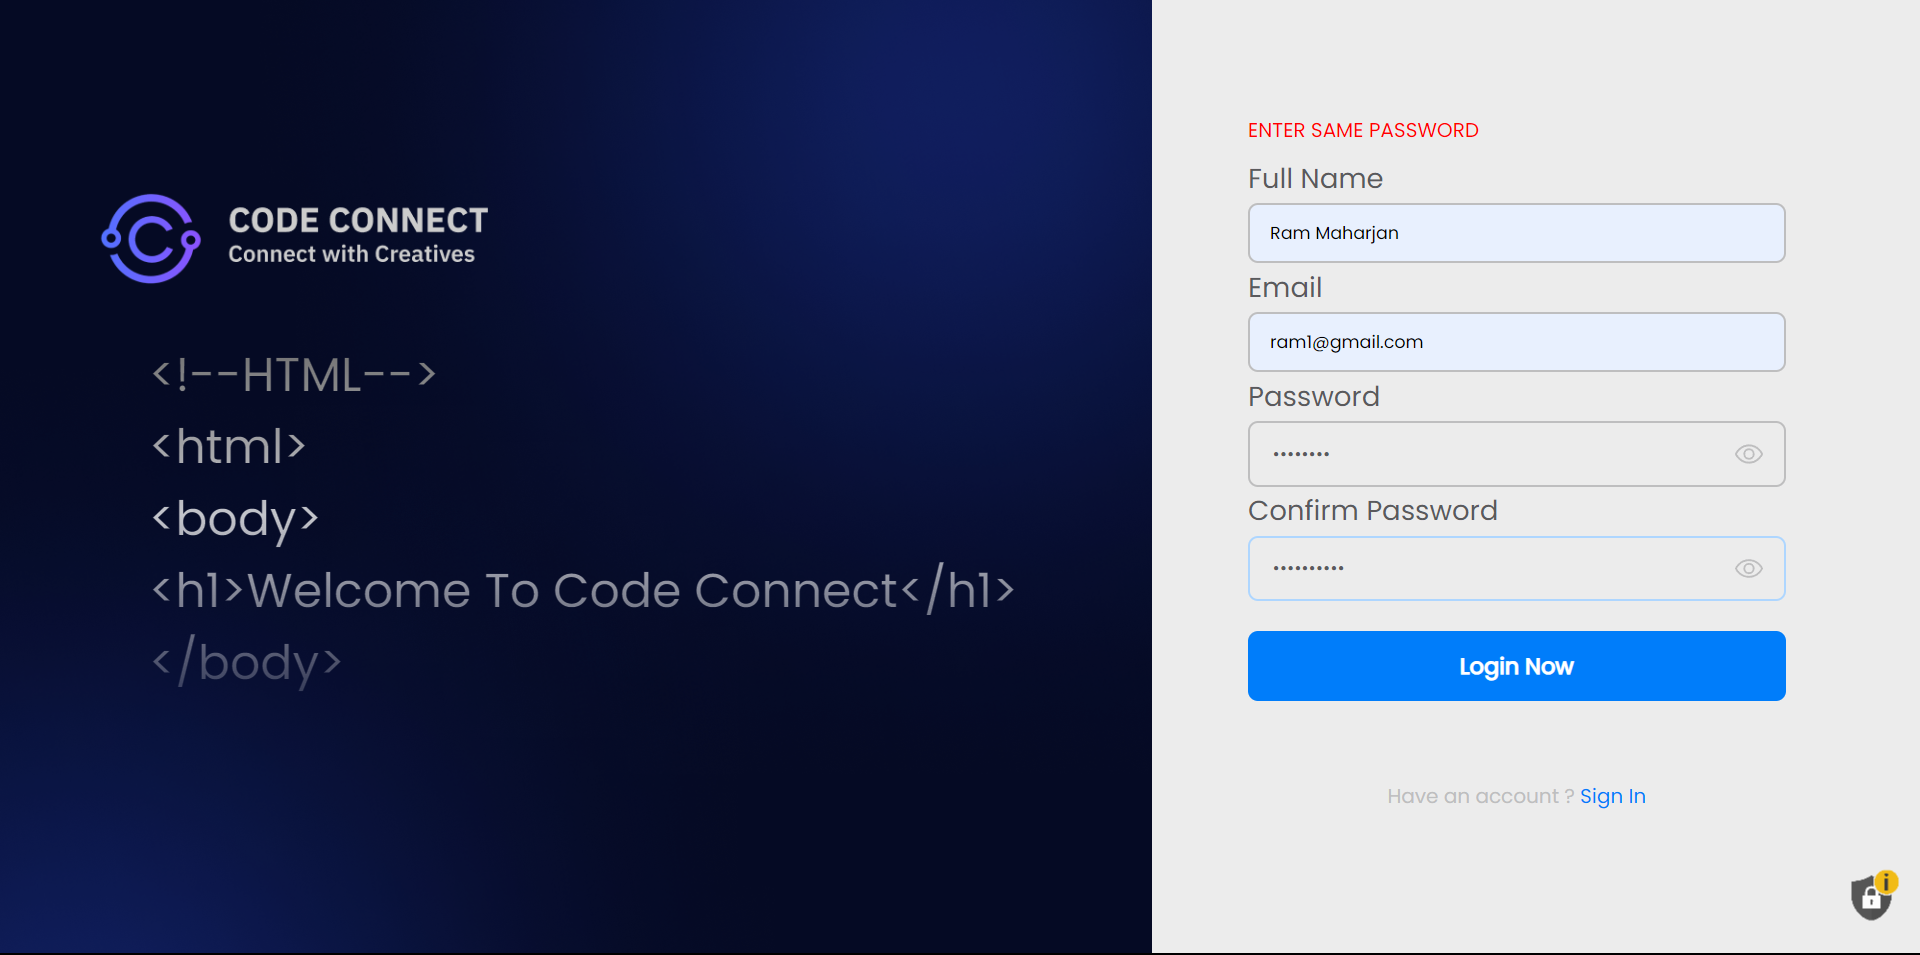
\includegraphics[width=1\textwidth]{4ImplementationAndTesting/screenshots/signup-pass-err.png}
%     \caption{Incorrect Confirm Password}
%     \label{fig: Incorrect Confirm Password}
% \end{figure}
% \begin{figure}[ht]
%     \centering
%     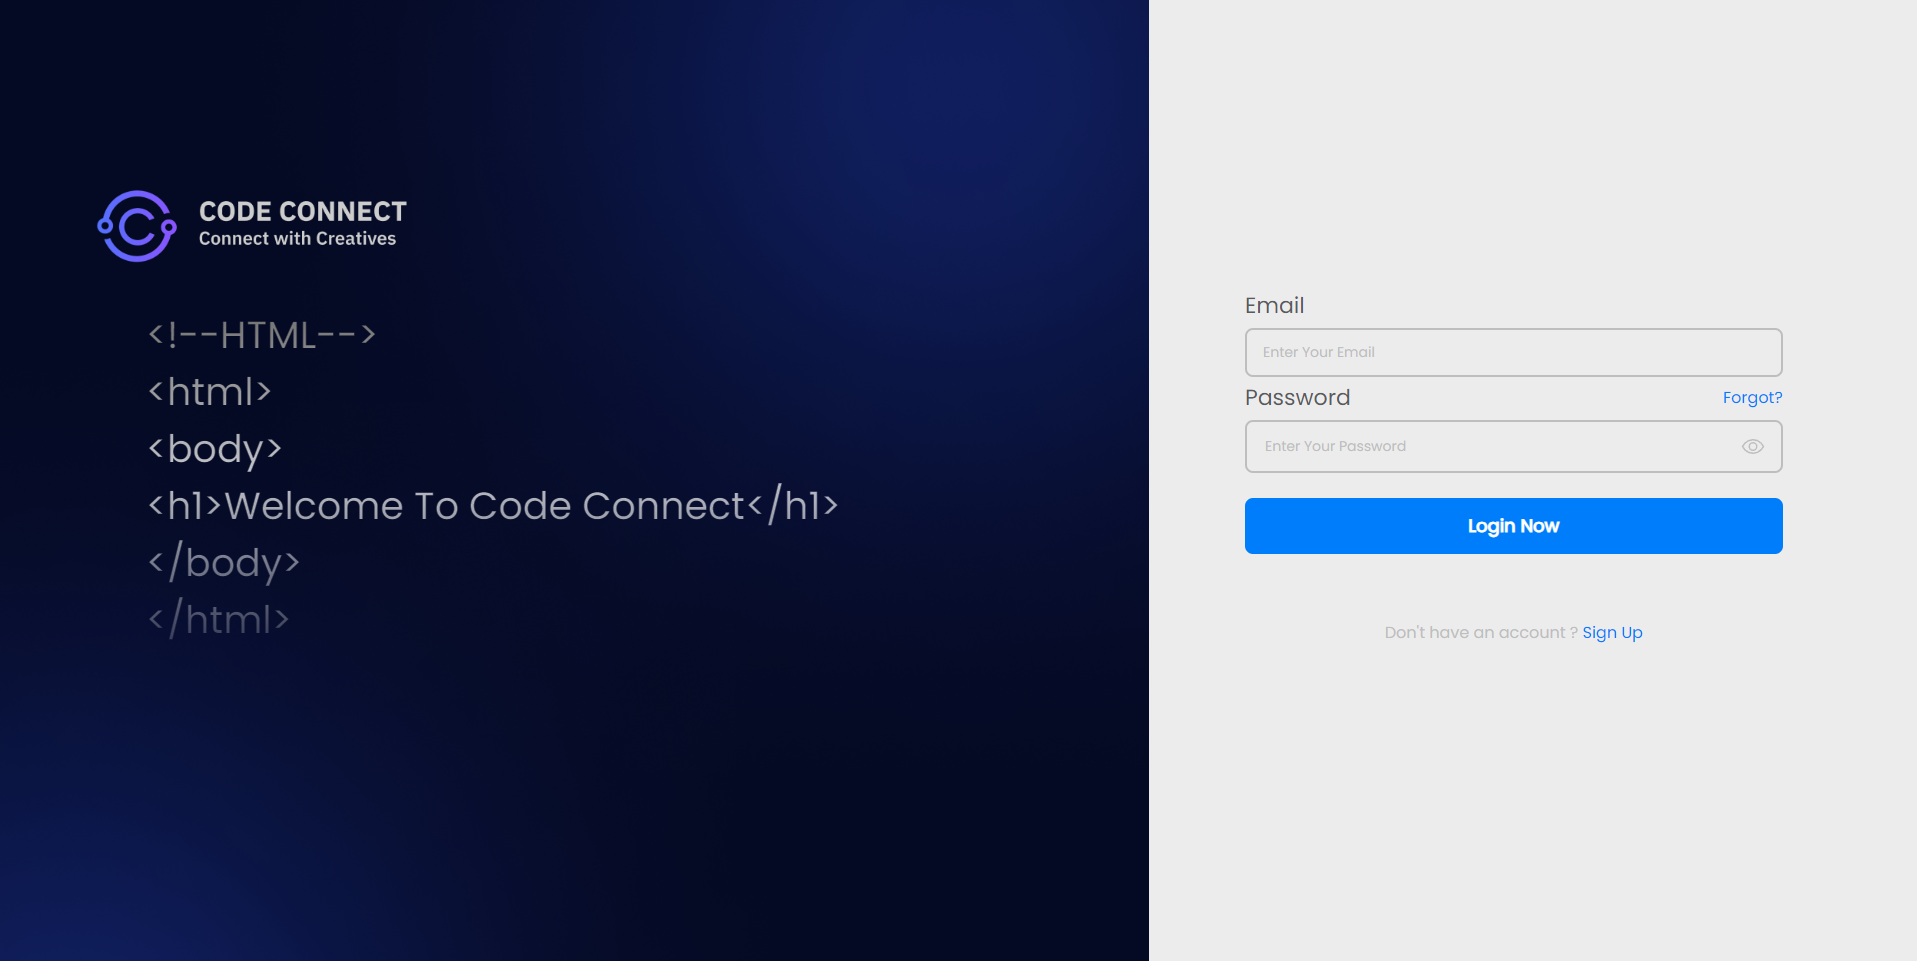
\includegraphics[width=1\textwidth]{ui_diagrams/desktop_login.png}
%     \caption{Correct SignUp Info Output}
%     \label{fig: Correct SignUp Info Output}
% \end{figure}
% \begin{figure}[ht]
%     \centering
%     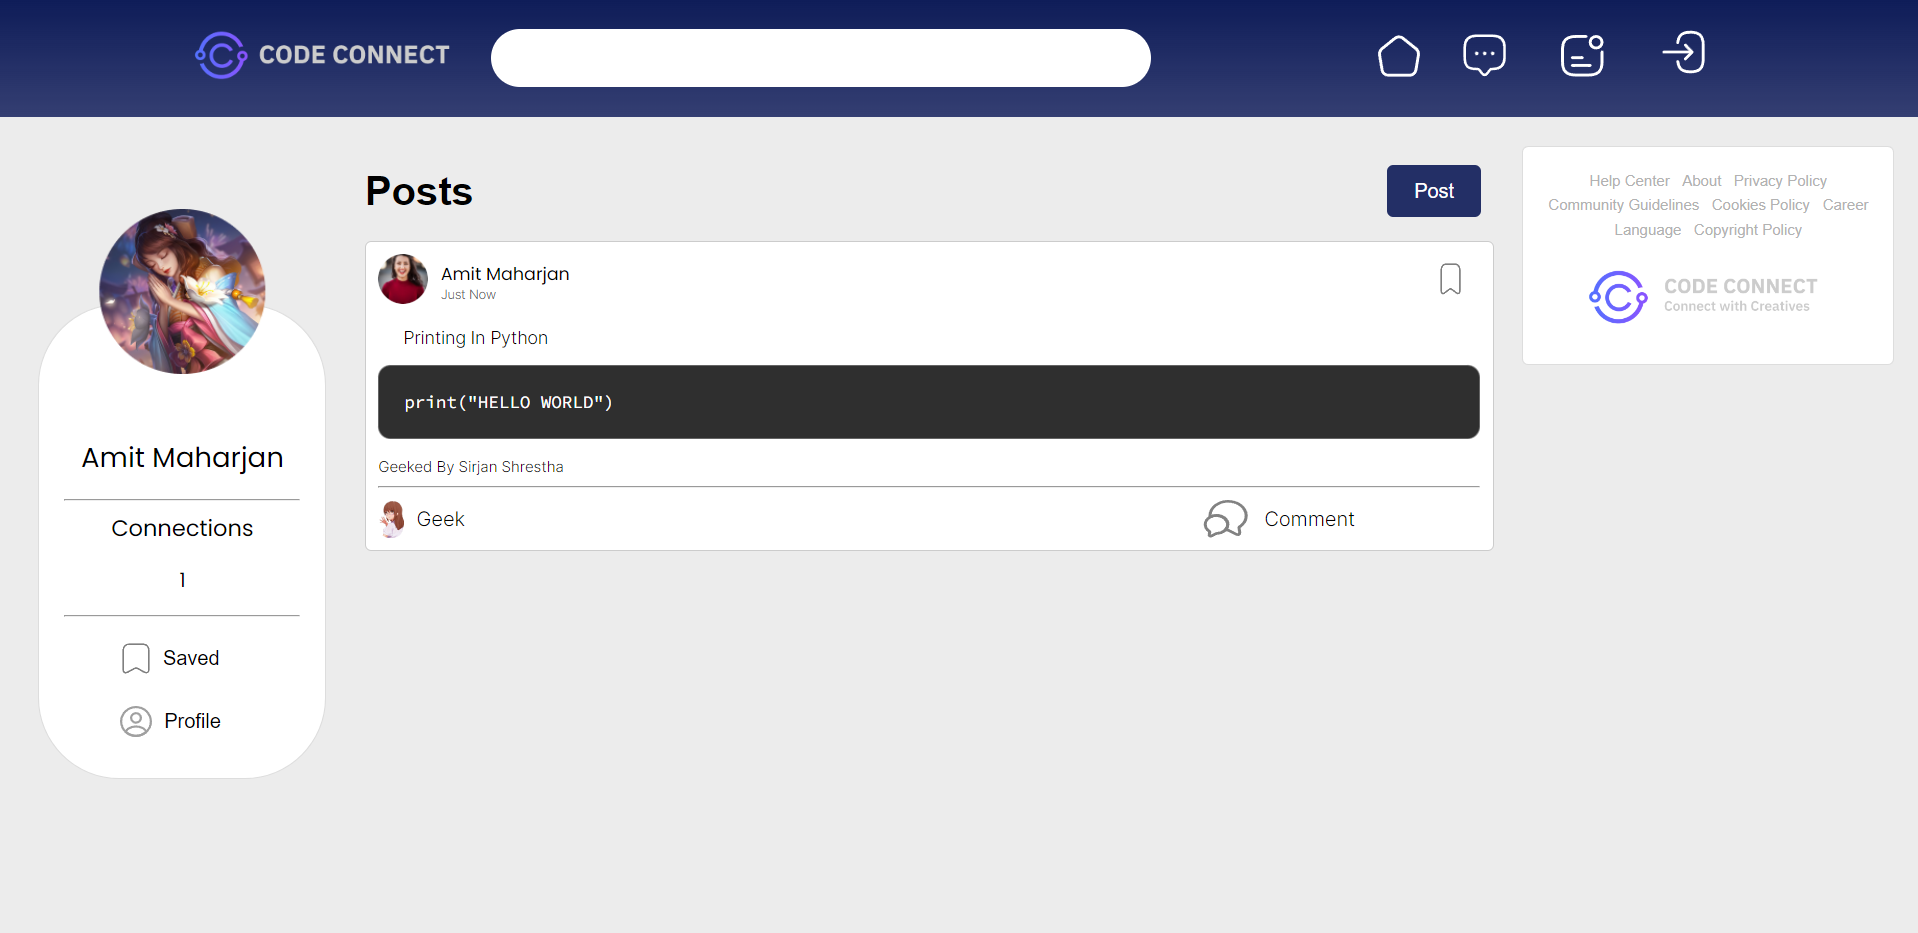
\includegraphics[width=1\textwidth]{ui_diagrams/desktop_homepage.png}
%     \caption{Correct Login Info Output}
%     \label{fig: Correct Login Info Output}
% \end{figure}


\chapter{CONCLUSION AND EXPECTED OUTCOMES}
\section{Conclusion}
Code Connect is a social networking web application designed specifically for creative it professionals. It should transform the way developers connect, collaborate, and learn from each other. The platform provides a range of features that allow creative it professionals to network, share knowledge, and enhance their skills. Code Connect also fosters a vibrant and inclusive resume and portfolio management system.

\section{Expected Outcome}
Code Connect is a platform that aims to create a thriving community of creative it professionals who can connect, collaborate, and learn from each other. The platform provides tailored features that facilitate meaningful interactions and knowledge exchange among its users. Through Code Connect, creative it professionals can expect to expand their professional network, gain insights from experienced peers, and receive support from the community. They can engage in discussions, seek advice, and offer assistance. Code Connect also aims to accelerate the professional growth of its users by providing access to valuable resources, tutorials, and learning opportunities. By connecting with like-minded individuals and staying up-to-date with the latest trends and technologies, creative it professionals can enhance their skills and advance their careers. The platform's expected outcome is to create a vibrant and supportive ecosystem that empowers creative it professionals and enriches their professional lives.
In this complex world of technologies new peoples who are intrested in the field of technology face alot of difficulties.
So they will also have exposure with the help of out technology.

% ================================Appendices Setup================================================


\begin{appendices}
\renewcommand\thechapter{A}
\renewcommand\thefigure{\thechapter.\arabic{figure}}
\chapter*{APPENDIX A}
\addtocontents{toc}{\textbf{APPENDIX A}}
\section{Project Schedule}
Below is the Gantt chart of our project Schedule to perfrom these specific tasks between these time frames.
\begin{figure}[H]
    \centering
        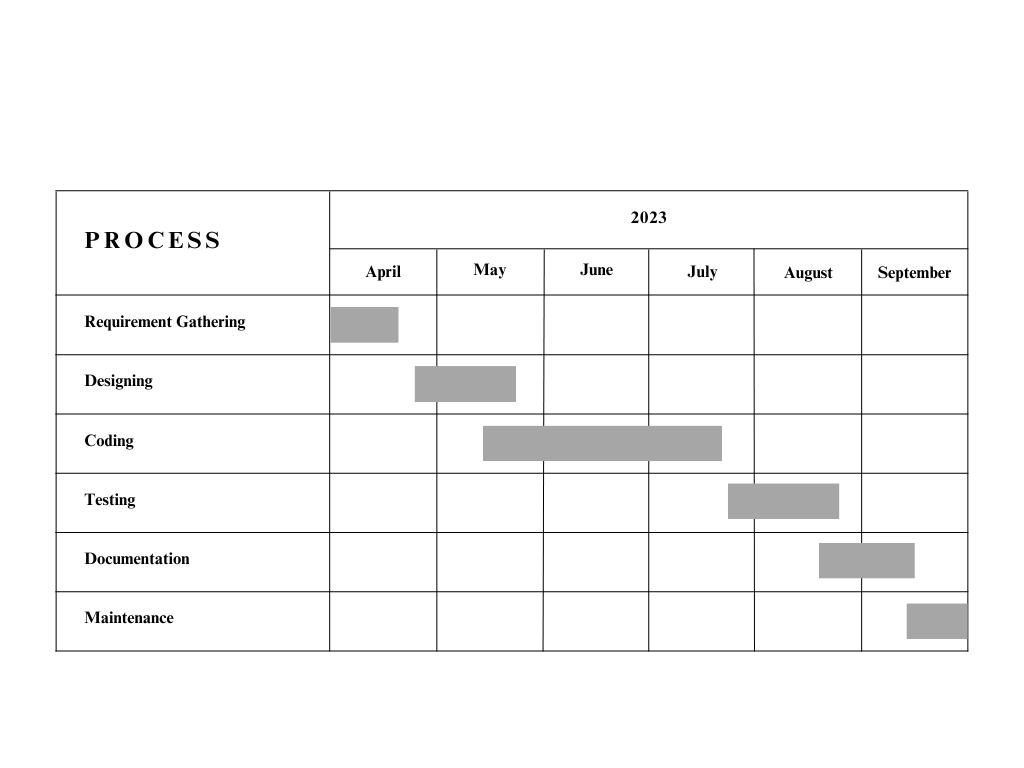
\includegraphics[width=400px]{Diagrams/Gantt_Chart.png}
    \caption{Gantt Chart of Schedule}
\end{figure}

\lstset{frame=tb,
  language=PHP,
  aboveskip=3mm,
  belowskip=3mm,
  showstringspaces=false,
  columns=flexible,
  basicstyle={\small\ttfamily},
  numbers=none,
  numberstyle=\tiny\color{gray},
  keywordstyle=\color{blue},
  commentstyle=\color{dkgreen},
  stringstyle=\color{mauve},
  breaklines=true,
  breakatwhitespace=true,
  tabsize=3
}
\section{Setup Guide to run Code Connect Locally}
\begin{enumerate}
    \item \textbf{Prerequisite:}
    \begin{enumerate}
        \item XAMPP
        \item Operating System that support XAMPP.
        \item Internet Connection for CDN libraries.
        \item Project Files Cloned from Git Hub.
    \end{enumerate}
    \item Clone Repo in htdocs/\\
    \begin{verbatim}
git clone https://github.com/sushantbramhacharya/CodeConnectBE.git
    \end{verbatim}
    \item Open PhpMyAdmin by going into \url{http://localhost/phpmyadmin}
    \item Create Database codeconnect
    \item Import Database codeconnect.sql from folder cloned using Import button located in navbar.
    \item Open XAMPP Control Panel.
    \item Start Apache and MySQL Servers.
    \item Run it on http://localhost/ or codeConnect directory.
\end{enumerate}
\section{Running Hosted Code Connect}
\begin{enumerate}
    \item Open Mobile/Desktop Browser .
    \item Go to \url{https://sushantbramhacharya.com.np/codeconnect}.
\end{enumerate}
\section{MySQL Connection in our CodeConnect PHP}
\vspace{1cm}
\begin{lstlisting}
    <?php
    $servername = "localhost";
    $username = "root";
    $password = "";
    $dbname = "codeconnect";

    $conn = new mysqli($servername, $username, $password, $dbname);

    if ($conn->connect_error) {
        die("Connection failed: " . $conn->connect_error);
    }
    ?>
    \end{lstlisting}
    \newpage
\section{JQuery AJAX Used in CodeConnect}
\vspace{1cm}
\begin{lstlisting}
    $.ajax({
    url: 'url',
    method: 'GET',
    data: { key1: 'value1', key2: 'value2' },
    dataType: 'json',
    success: function(response) {
        console.log(response);
    },
    error: function(xhr, status, error) {
        console.log('Error: ' + error);
    }
    });

    \end{lstlisting}
    \section{Database Screenshots}
    Here the Screenshots of tables used in database of code connect.
    \begin{figure}[H]
        \centering
            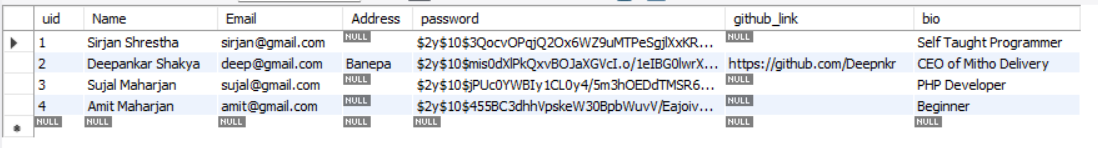
\includegraphics[width=420px]{db_img/user.png}
        \caption{User Table}
    \end{figure}
    \begin{figure}[H]
        \centering
            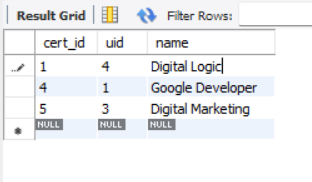
\includegraphics[width=150px]{db_img/certifications.png}
        \caption{Certifications Table}
    \end{figure}
    \begin{figure}[H]
        \centering
            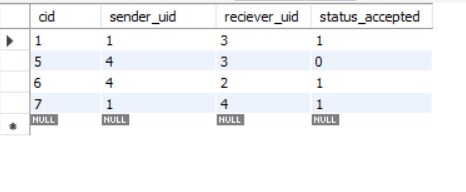
\includegraphics[width=200px]{db_img/connections.png}
        \caption{Connections Table}
    \end{figure}
    
    \begin{figure}[H]
        \centering
            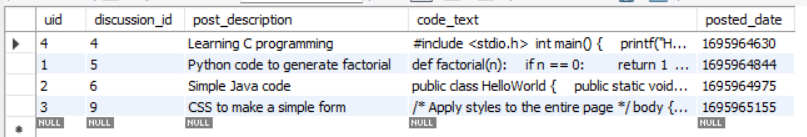
\includegraphics[width=400px]{db_img/discussion.png}
        \caption{Discussion Table}
    \end{figure}
    
    \begin{figure}[H]
        \centering
            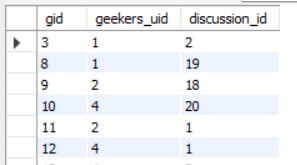
\includegraphics[width=170px]{db_img/geek.png}
        \caption{Geek Table}
    \end{figure}
    
    \begin{figure}[H]
        \centering
            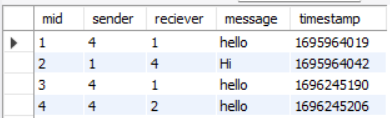
\includegraphics[width=200px]{db_img/messages.png}
        \caption{Messages Table}
    \end{figure}
    
    \begin{figure}[H]
        \centering
            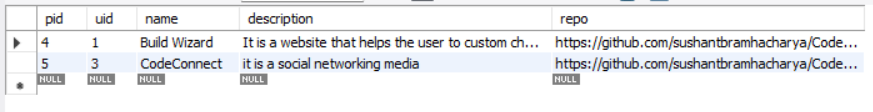
\includegraphics[width=400px]{db_img/projects.png}
        \caption{Projects Table}
    \end{figure}
    
    \begin{figure}[H]
        \centering
            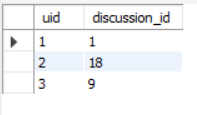
\includegraphics[width=150px]{db_img/saved.png}
        \caption{Saved Table}
    \end{figure}
    
    \begin{figure}[H]
        \centering
            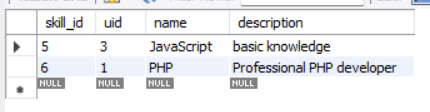
\includegraphics[width=220px]{db_img/skills.png}
        \caption{Skills Table}
    \end{figure}
    
    \begin{figure}[H]
        \centering
            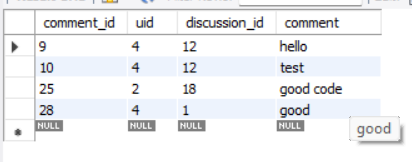
\includegraphics[width=200px]{db_img/comments.png}
        \caption{Comments Table}
    \end{figure}
\section{Supervisor Consultation Form}
\begin{figure}[H]
    \centering
    \includegraphics[width=400px]{Appendix/supervisor-form.jpg}
    \caption{Supervisor Consultation Form}
\end{figure}



\section{Remaining Part}

\end{appendices}



%========================References setup=========================================================
\newpage
\bibliographystyle{unsrt}
\bibliography{References/references}

\addcontentsline{toc}{chapter}{REFERENCES}

%=============================================================================================



%=========================================================================
\end{document}